%% Extended results (full version of the supplementary analyses)
%% Generated from the long supplement; the short supplement cites sections E1--E9.
%% Companion to: Filling the gaps: matrix completion imputation
%% for broader gene coverage in cross-dataset full-merge
%% expression analysis
%%
%% Compile: pdflatex supplement.tex  (twice, for refs)

\documentclass[11pt,a4paper]{article}

\usepackage[margin=1in]{geometry}
\usepackage{amsmath}
\usepackage{amssymb}
\usepackage[section]{placeins}
\usepackage{graphicx}
\usepackage{booktabs}
\usepackage{array}
\usepackage{tabularx}
\usepackage{url}
\usepackage{xcolor}
\usepackage[authoryear,round]{natbib}
\usepackage{hyperref}
\hypersetup{colorlinks=true,linkcolor=blue,citecolor=blue,urlcolor=blue}
\setlength{\emergencystretch}{1em}
\renewcommand{\topfraction}{0.85}
\renewcommand{\bottomfraction}{0.85}
\renewcommand{\textfraction}{0.10}
\renewcommand{\floatpagefraction}{0.75}

% S-prefix numbering
\renewcommand{\thefigure}{E\arabic{figure}}
\renewcommand{\thetable}{E\arabic{table}}
\renewcommand{\thesection}{E\arabic{section}}

\title{Extended results:\\
  Filling the gaps: matrix completion imputation for broader
  gene coverage when merging microarray gene expression datasets}

\author{Oleksandr Lykhenko, Yehor Polyakov, Maria Obolenskaya}

\date{}

\begin{document}

\maketitle

\tableofcontents

\noindent This document holds the full tables, figures and protocols
behind the article and its Supplementary Materials, which report
one table and at most one figure per analysis and cite the
sections below as E1--E9. Section titles that mention the main
text refer to the long version of the article.

\section*{What this document answers}
\addcontentsline{toc}{section}{What this document answers}

\noindent
\begin{tabularx}{\textwidth}{@{}lX@{}}
\toprule
\textbf{E1} & \textbf{How accurately are masked values reconstructed, and by
  which imputer?} Seven imputers under three masking schemes.
  \emph{Reached from} Methods, \emph{Matrix completion} and
  \emph{Masking schemes for holdout validation}; Discussion,
  \emph{Limitations}. \\
\addlinespace
\textbf{E2} & \textbf{Does designating a reference batch change what ComBat
  produces?} Corrected values compared with standard ComBat.
  \emph{Reached from} Results, \emph{Batch correction}. \\
\addlinespace
\textbf{E3} & \textbf{How stable is the DEG list when the samples are
  resampled, and is it more than noise?} Sample-size convergence,
  a label-permutation null, a balanced two-dataset reference, and
  split-half.
  \emph{Reached from} Results, \emph{Subsampling validation}. \\
\addlinespace
\textbf{E4} & \textbf{Do the gained genes agree with the earlier
  single-platform analysis?} A consistency check, not external
  corroboration --- the two cohorts share 16 of 22 samples.
  \emph{Reached from} Results, \emph{Biological plausibility of gained genes}. \\
\addlinespace
\textbf{E5} & \textbf{When the pipeline calls an imputed gene differentially
  expressed, is the call right?} The holdout experiment: three masking
  schemes, both ComBat variants, seven imputers, and the
  Reference/Masked/Oracle decomposition. \emph{Reached from} Results,
  \emph{Holdout validation of differential expression on imputed genes};
  Methods, \emph{Masking schemes for holdout validation}. \\
\addlinespace
\textbf{E6} & \textbf{Is the disagreement with RNA-seq a matter of technology
  or of gestational age?} A gestational-age-matched re-run of the Prater
  comparison. \emph{Reached from} Results, \emph{Cross-technology
  concordance with independent RNA-seq data}. \\
\addlinespace
\textbf{E7} & \textbf{Does the choice of biological covariate in ComBat change
  the result?} Four specifications, on the full cohort and under subsampling.
  \emph{Reached from} Results, \emph{Sensitivity to ComBat biological
  covariate specification}. \\
\addlinespace
\textbf{E8} & \textbf{How many genes does each coverage threshold recover, and
  at what cost in missingness?} \emph{Reached from} Results,
  \emph{Gene recovery and missingness}; Figure~1's caption. \\
\addlinespace
\textbf{E9} & \textbf{How many DEGs does each imputation and normalization
  combination give?} \emph{Reached from} Results,
  \emph{Differential expression}. \\
\bottomrule
\end{tabularx}

\bigskip

%% -----------------------------------------------------------------
\section{Imputation accuracy: full cross-validation results}
\label{sec:supp-imputation}
%% -----------------------------------------------------------------

Under the gene--dataset block masking that a cross-platform merge
produces, most of the reconstruction accuracy comes from centering
the data: a fill that only centres every gene and every sample
closes about $88\%$ of the gap between the gene-mean baseline and
the best method, and every method that works on the centered
matrix lands within about $0.1$ RMSE of the others. Under
random-cell masking the methods separate.
Table~\ref{tab:supp-imputation} reports seven imputers on all
three schemes; Figure~\ref{fig:supp-cv-range} plots each method's
best-to-worst RMSE range against two no-skill anchors.

Accuracy was quantified by leave-out cross-validation
under the three masking schemes defined in the Methods
(random cells, gene--dataset block, worst-case block): in each
repeat 10\% of the observed cells (${\sim}144{,}800$ of
$1{,}447{,}937$) were masked, every imputer filled the same
masked cells, and the filled values were compared with the
truth. Three repeats were run per scheme, each with a freshly
drawn, seeded mask. The masks are the same ones that
Section~\ref{sec:supp-blockholdout} carries through batch
correction and differential expression, so the accuracy of the
imputed \emph{values} reported here and the accuracy of the
\emph{calls} reported there refer to identical masked cells.
Three metrics are reported, the standard accuracy measures of
the microarray imputation literature \citep{Troyanskaya2001}:
\begin{itemize}
  \item \emph{Pearson $r$} --- correlation between imputed and
    true values across the masked cells; unit-free, $r = 1$
    perfect and $r = 0$ chance.
  \item \emph{RMSE} (root-mean-square error) ---
    $\sqrt{\frac{1}{n}\sum_{ij}(\hat x_{ij} - x_{ij})^2}$,
    where the sum runs over the $n$ masked cells $(i,j)$.
    Because the per-dataset expression matrices entering the
    pipeline are already log$_2$-transformed, RMSE is in units
    of $\log_2$ expression; for scale, the observed values have
    a standard deviation of $2.85$ log$_2$ units, so an RMSE of
    $0.60$ (\textit{softImpute}, random cells) is an error of
    ${\sim}21\%$ of the expression variability. Squaring makes RMSE the more sensitive of the
    two to a few badly imputed cells.
  \item \emph{MAE} (mean absolute error) ---
    $\frac{1}{n}\sum_{ij}|\hat x_{ij} - x_{ij}|$ over the same
    cells, also in $\log_2$ units, weighting every error
    linearly.
\end{itemize}

\paragraph{Block masking is the informative benchmark.}
Random-cell masking --- individual observed cells drawn
uniformly at random --- is the classical in-distribution
leave-out, and it is easy: a masked cell almost always sits in a dataset
where the same gene is observed in other samples, and
\textit{softImpute} recovers it to within ${\sim}21\%$ of the
expression standard deviation. The gene--dataset block mask
removes an entire gene$\times$dataset block, drawn among the
genes observed in all six datasets, which is the
missingness a cross-platform merge actually produces --- an
entire gene absent from an entire dataset --- and accuracy
drops to about half an expression standard deviation. The
\emph{worst-case block} mask stresses coverage instead of
pattern: every selected gene is masked down to
$n_{\min} = 2$ randomly chosen datasets (one above the
pipeline's actual floor of a single dataset), with a random
subset of genes selected per repeat so that the masked
fraction stays at 10\%. \textit{softImpute} lands there within
$0.1$ RMSE of its gene--dataset block result, with zero
convergence failures across all repeats, so accuracy degrades
gracefully rather than catastrophically as coverage falls.

\paragraph{Choice of the softImpute $\lambda$.}
The number of latent factors \textit{softImpute} keeps is set by
the shrinkage $\lambda$, which was chosen by hold-out on the
pattern that matters. The production warm-start path (eight
geometric steps from $\lambda_0$, where every factor is shrunk
to zero, to $0.01\lambda_0$) was fitted on three gene--dataset
block masks drawn with their own seeds, and on three random-cell
masks for comparison, and the masked cells were scored at every
step (Table~\ref{tab:supp-lambda-path}). The selection masks
share 14--16\% of their cells with the validation masks of
Table~\ref{tab:supp-imputation}, the chance level for two
independent draws being 15\%, so the accuracy reported here is
not measured on the cells that chose $\lambda$. Block error
falls steeply over the first steps, reaches its minimum at step~3
($\lambda = 104.2$, 13 factors; RMSE $1.517 \pm 0.018$, mean
$\pm$ SE over the three masks) and rises slowly as more factors
enter. By the one-standard-error rule \citep{Hastie2009} the
largest $\lambda$ whose error lies within one SE of the minimum
is step~2 ($\lambda = 201.3$, 5 factors, RMSE $1.520$), the
setting used throughout; the rank cap of 60 does not bind
there. The SE mostly reflects how hard each mask is: compared
within masks, step~3 is better than step~2 on all three, by
$0.003$, or $0.2\%$ of the error. Random-cell masks favor many
more factors (lowest error at step~5, where the cap of 60
binds), because a scattered masked cell keeps its gene's other
measurements in the same dataset; the chosen setting gives up
accuracy on such isolated cells (RMSE $0.60$ against $0.33$ at
that minimum) for accuracy on the block pattern that
cross-platform merging produces.

\begin{table}[htbp]
\centering
\footnotesize
\begin{tabular}{@{}rrrrccc@{}}
\toprule
\textbf{Step} & $\boldsymbol{\lambda}$ & $\boldsymbol{\lambda/\lambda_0}$ & \textbf{Factors} & \textbf{Block RMSE} & \textbf{Block $r$} & \textbf{Random-cell RMSE} \\
\midrule
0 & 750.2 & 1.000 & 1 & $1.587 \pm 0.018$ & $0.799$ & $1.074 \pm 0.002$ \\
1 & 388.6 & 0.518 & 2 & $1.547 \pm 0.019$ & $0.808$ & $0.861 \pm 0.001$ \\
2 & 201.3 & 0.268 & \textbf{5} & $1.520 \pm 0.018$ & $0.814$ & $0.598 \pm 0.001$ \\
3 & 104.2 & 0.139 & 13 & $1.517 \pm 0.018$ & $0.815$ & $0.445 \pm 0.001$ \\
4 &  54.0 & 0.072 & 35 & $1.518 \pm 0.018$ & $0.815$ & $0.361 \pm 0.001$ \\
5 &  28.0 & 0.037 & 60 & $1.526 \pm 0.018$ & $0.814$ & $0.328 \pm 0.000$ \\
6 &  14.5 & 0.019 & 60 & $1.534 \pm 0.018$ & $0.812$ & $0.332 \pm 0.000$ \\
7 &   7.5 & 0.010 & 60 & $1.543 \pm 0.018$ & $0.810$ & $0.353 \pm 0.000$ \\
\bottomrule
\end{tabular}
\caption{The \textit{softImpute} warm-start $\lambda$ path on
  the selection masks (three gene--dataset block masks and three
  random-cell masks, 10\% of the observed cells each, seeds
  1001--1003). Factors: number of non-zero singular values of the
  fit on the unmasked matrix. Errors are mean $\pm$ SE over the
  three masks, in $\log_2$ units. Bold: the step selected by the
  one-standard-error rule on block RMSE (step~2); the lowest block
  error is at step~3.}
\label{tab:supp-lambda-path}
\end{table}

\paragraph{Centering does most of the work.}
Every method in Table~\ref{tab:supp-imputation} except the two
means starts from the same step: the \texttt{biScale} model
\citep{Hastie2015} estimates a center and a scale for every gene
and every sample from the observed cells, the imputer fills the
centered matrix, and the centering is then undone. The
\emph{biScale fill} stops after the first step and fills every gap
with the gene center plus the sample offset --- \textit{softImpute}
with zero factors. Under gene--dataset block masking it reaches
RMSE $1.56$, against $2.54$ for the gene mean (which has the gene
center but no sample offset) and $1.43$ for the best method;
centering alone thus accounts for
$(2.54 - 1.56)/(2.54 - 1.43) \approx 88\%$ of the achievable
reduction. The four methods built on the centered matrix ---
\textit{softImpute} (5 factors), imputePCA (20 components, chosen
by the same hold-out rule; Methods), and nearest-neighbor
imputation over genes or over samples ($k = 10$) --- span RMSE
$1.43$--$1.53$ ($r = 0.815$--$0.836$) under block masking and
$1.51$--$1.63$ under the worst-case mask: within about $0.1$
log$_2$ units of each other, against repeat SDs of
$0.01$--$0.03$. Under random-cell masking they separate (RMSE
$0.32$ for imputePCA, $0.50$ for the two KNN variants, $0.60$ for
\textit{softImpute}, against $1.07$ for the biScale fill),
because a scattered masked cell keeps the gene's other
measurements in the same dataset, and the residual pattern the
methods model is then most of what is left to recover.
\textit{softImpute}'s setting ranks last of the four there, the
price of choosing $\lambda$ on block masks
(Table~\ref{tab:supp-lambda-path}). Without the centering step the
same neighbor methods are much worse on blocks (RMSE $1.98$ for
gene-space and $2.31$ for sample-space KNN on the uncentered
matrix, in the companion outputs), and imputePCA on uncentered
input reaches at best $1.89$ on the selection masks
(Methods); these variants are not reported further. imputePCA is
also slow: a fit on this matrix takes about 16 minutes, its EM
loop running to the package's 1{,}000-iteration cap, against under
a minute for \textit{softImpute}.

\paragraph{The mean baselines.}
The \emph{gene mean} baseline fills every missing cell for a
gene with that gene's mean over all samples in which it was
observed, regardless of dataset; the \emph{batch mean} baseline
uses the gene's mean \emph{within the same dataset}, preserving
dataset-specific expression levels, and falls back to the gene
mean when the gene is absent from that dataset altogether.
Batch mean is accordingly strong under random-cell masking (RMSE
$0.44$, better than \textit{softImpute}'s block-tuned setting) and
collapses onto gene mean under both block schemes --- identical
values, because holding out a whole gene--dataset block leaves
no within-dataset observation for the fallback to use. Neither
carries the sample's own level, which is why both fall far
behind the biScale fill exactly where cross-platform merging
needs an imputer to work.
Figure~\ref{fig:supp-cv-range} sets every method against two
no-skill anchors computed from the observed cells of the merged
matrix: predicting one overall mean for every masked cell
gives RMSE $2.85$, equal to the overall expression SD, and
predicting each dataset's own overall mean gives $2.03$, so the
gap between the two anchors is the part of the error
attributable to between-dataset offsets alone. That
\emph{per-dataset mean} is a single number per dataset and is
not the \emph{batch mean} baseline, which predicts each gene's
within-dataset mean.

\paragraph{Accuracy by what the gene was left with.}
Section~\ref{sec:supp-blockholdout} shows that the fate of a
masked gene in differential expression depends on whether it
retains a real measurement in the ComBat reference batch
(GSE100051). Table~\ref{tab:supp-imputation-pergene} therefore
reports reconstruction error per gene --- the mean absolute
error over a gene's masked cells, then the median over genes,
as mean $\pm$ SD across the three repeats --- split by that
same criterion. Random-cell masking is omitted because it
never removes a gene's entire reference block. For
\textit{softImpute} the two strata differ by only about
$0.2$ log$_2$ units, and not even in a consistent direction:
under gene--dataset block masking genes that lose the
reference batch are reconstructed slightly worse ($0.99$ vs
$0.76$), under the worst-case mask slightly better ($0.83$ vs
$0.98$), the latter because genes kept down to two datasets
are, on average, better reconstructed when neither of the two
is the largest batch. Imputed values are therefore recovered
about equally well regardless of which datasets survive; as
Section~\ref{sec:supp-blockholdout} shows, differential
expression built on them is not.

\begin{figure}[htbp]
\centering
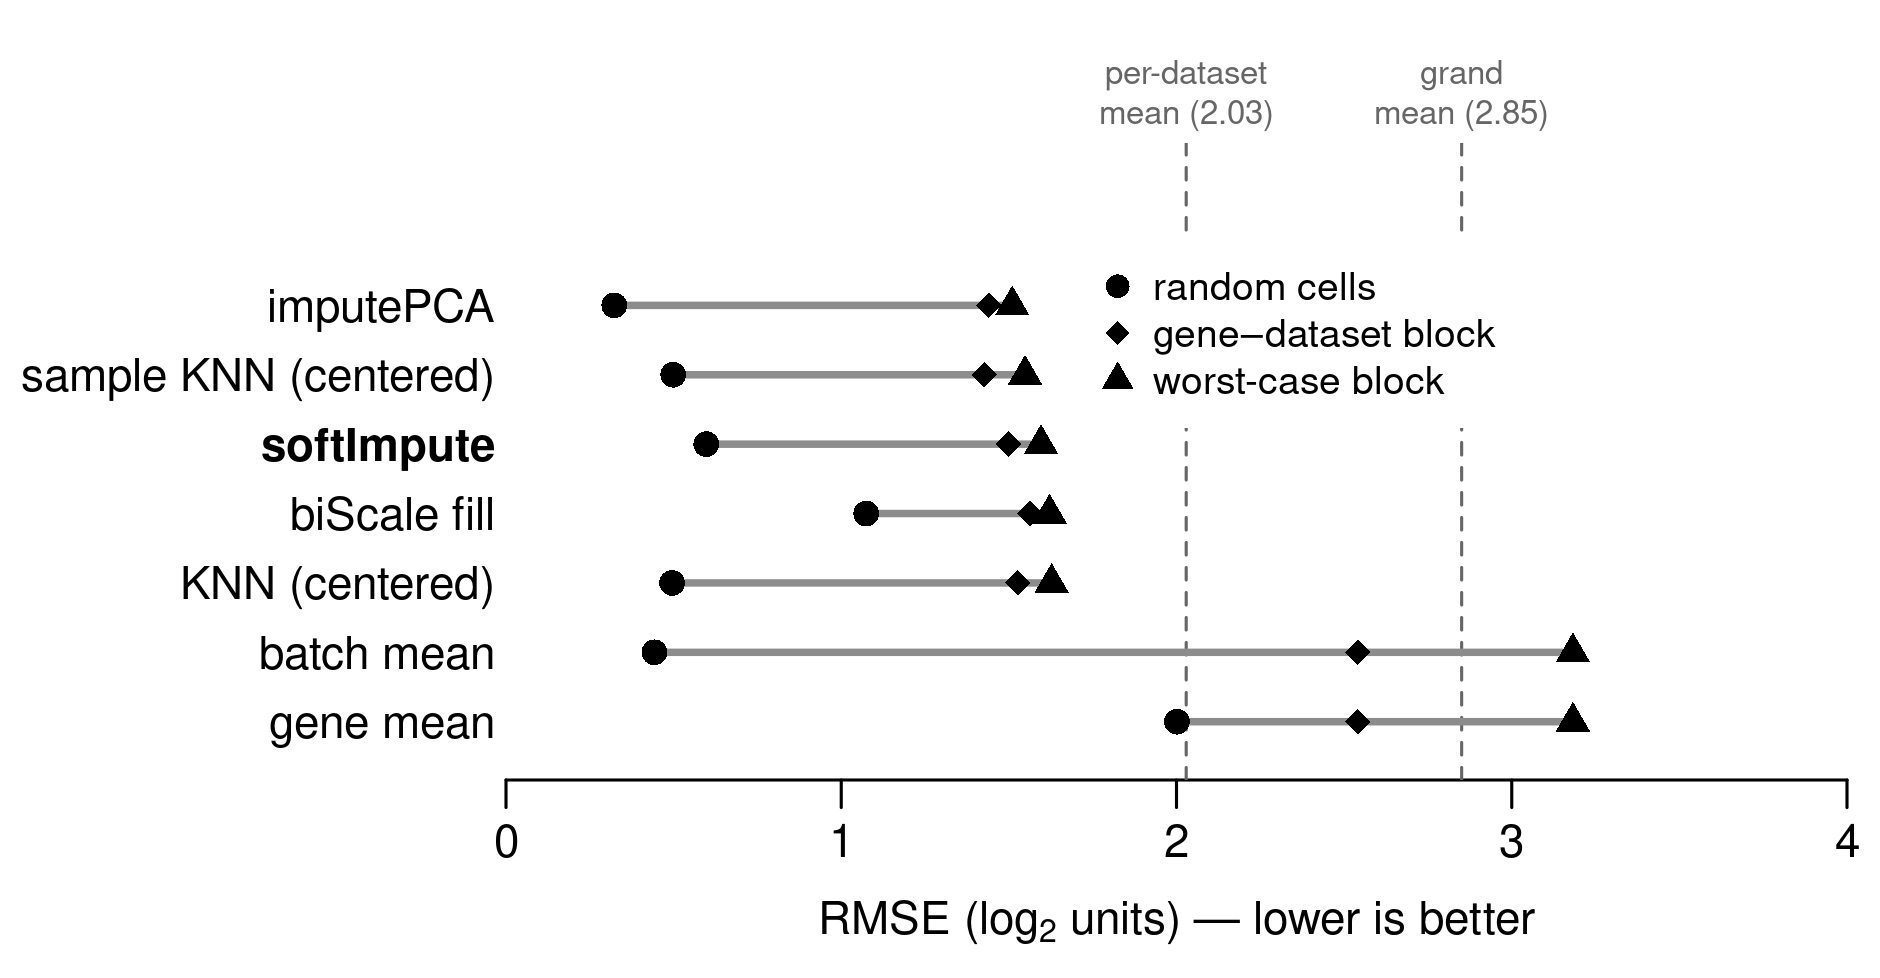
\includegraphics[width=\textwidth]{figures/fig_imputation_cv_range.png}
\caption{Imputation cross-validation as a range plot --- a
  rendering of Table~\ref{tab:supp-imputation}. Each line spans
  one method's best-to-worst RMSE across the three masking
  protocols ($\bullet$ random cells, $\blacklozenge$
  gene--dataset block, $\blacktriangle$ worst-case block);
  methods are ordered by worst-case RMSE. All standard
  deviations are $\le 0.04$ log$_2$ units, smaller than the
  markers. The two dashed lines are the no-skill anchors
  defined in the text: \emph{grand mean} ($2.85$) and
  \emph{per-dataset mean} ($2.03$).}
\label{fig:supp-cv-range}
\end{figure}

\begin{table}[htbp]
\centering
\footnotesize
\begin{tabular}{@{}llrccc@{}}
\toprule
\textbf{Masking} & \textbf{Method} & \textbf{Cells masked} & \textbf{Pearson $r$} & \textbf{RMSE} & \textbf{MAE} \\
\midrule
random cells & softImpute & 144{,}794 & $0.978 \pm 0.000$ & $0.597 \pm 0.001$ & $0.425 \pm 0.001$ \\
 & imputePCA & 144{,}794 & $0.994 \pm 0.000$ & $0.323 \pm 0.001$ & $0.216 \pm 0.000$ \\
 & KNN (centered) & 144{,}794 & $0.985 \pm 0.000$ & $0.496 \pm 0.002$ & $0.325 \pm 0.001$ \\
 & sample KNN (centered) & 144{,}794 & $0.985 \pm 0.000$ & $0.499 \pm 0.001$ & $0.318 \pm 0.001$ \\
 & biScale fill & 144{,}794 & $0.926 \pm 0.000$ & $1.074 \pm 0.002$ & $0.786 \pm 0.002$ \\
 & gene mean & 144{,}794 & $0.713 \pm 0.000$ & $2.001 \pm 0.001$ & $1.445 \pm 0.001$ \\
 & batch mean & 144{,}794 & $0.988 \pm 0.000$ & $0.443 \pm 0.001$ & $0.299 \pm 0.000$ \\
\addlinespace
gene--dataset block & softImpute & 144{,}811 & $0.820 \pm 0.002$ & $1.499 \pm 0.011$ & $1.148 \pm 0.007$ \\
 & imputePCA & 144{,}811 & $0.834 \pm 0.005$ & $1.439 \pm 0.021$ & $1.094 \pm 0.004$ \\
 & KNN (centered) & 144{,}811 & $0.815 \pm 0.006$ & $1.527 \pm 0.028$ & $1.158 \pm 0.017$ \\
 & sample KNN (centered) & 144{,}811 & $0.836 \pm 0.004$ & $1.426 \pm 0.016$ & $1.083 \pm 0.006$ \\
 & biScale fill & 144{,}811 & $0.806 \pm 0.002$ & $1.563 \pm 0.010$ & $1.203 \pm 0.006$ \\
 & gene mean & 144{,}811 & $0.358 \pm 0.002$ & $2.541 \pm 0.020$ & $1.957 \pm 0.019$ \\
 & batch mean & 144{,}811 & $0.358 \pm 0.002$ & $2.541 \pm 0.020$ & $1.957 \pm 0.019$ \\
\addlinespace
worst-case block & softImpute & 144{,}858 & $0.824 \pm 0.004$ & $1.596 \pm 0.015$ & $1.203 \pm 0.013$ \\
 & imputePCA & 144{,}858 & $0.842 \pm 0.006$ & $1.510 \pm 0.025$ & $1.133 \pm 0.015$ \\
 & KNN (centered) & 144{,}858 & $0.818 \pm 0.003$ & $1.627 \pm 0.013$ & $1.228 \pm 0.014$ \\
 & sample KNN (centered) & 144{,}858 & $0.834 \pm 0.005$ & $1.548 \pm 0.022$ & $1.166 \pm 0.014$ \\
 & biScale fill & 144{,}858 & $0.819 \pm 0.004$ & $1.621 \pm 0.014$ & $1.223 \pm 0.013$ \\
 & gene mean & 144{,}858 & $0.342 \pm 0.010$ & $3.182 \pm 0.039$ & $2.567 \pm 0.030$ \\
 & batch mean & 144{,}858 & $0.342 \pm 0.010$ & $3.182 \pm 0.039$ & $2.567 \pm 0.030$ \\
\bottomrule
\end{tabular}
\caption{Leave-out cross-validation of imputation accuracy
  (6 datasets, 17{,}531 genes). The seven
  imputers and the three masking schemes are defined at the
  start of this section. All rows show the mean $\pm$ SD over three
  repeats; within a repeat every method fills the same masked
  cells, so the comparison is mask-matched across methods and
  across the differential expression holdout of
  Section~\ref{sec:supp-blockholdout}. ``Cells masked'' is the
  mean number of masked entries per repeat; gene mean and
  batch mean coincide under both block schemes because holding
  out a whole gene--dataset block leaves the batch mean nothing
  to average. KNN and sample KNN are run on the
  \texttt{biScale}-centered matrix; on the uncentered matrix their
  block RMSE is $1.98$ and $2.31$ (companion outputs).}
\label{tab:supp-imputation}
\end{table}

\begin{table}[htbp]
\centering
\footnotesize
\begin{tabular}{@{}llrrcc@{}}
\toprule
\textbf{Masking} & \textbf{Method} & \multicolumn{2}{c}{\textbf{Genes}} & \multicolumn{2}{c}{\textbf{Median per-gene MAE}} \\
\cmidrule(lr){3-4}\cmidrule(lr){5-6}
 & & \textbf{ref.\ kept} & \textbf{ref.\ masked} & \textbf{ref.\ kept} & \textbf{ref.\ masked} \\
\midrule
gene--dataset block & softImpute & 3{,}911 & 1{,}246 & $0.76 \pm 0.01$ & $0.99 \pm 0.02$ \\
 & imputePCA & 3{,}911 & 1{,}246 & $0.74 \pm 0.00$ & $0.93 \pm 0.01$ \\
 & KNN (centered) & 3{,}911 & 1{,}246 & $0.71 \pm 0.01$ & $0.99 \pm 0.01$ \\
 & sample KNN (centered) & 3{,}911 & 1{,}246 & $0.71 \pm 0.00$ & $0.93 \pm 0.01$ \\
 & biScale fill & 3{,}911 & 1{,}246 & $0.90 \pm 0.01$ & $1.01 \pm 0.02$ \\
 & gene mean & 3{,}911 & 1{,}246 & $2.61 \pm 0.02$ & $1.34 \pm 0.02$ \\
 & batch mean & 3{,}911 & 1{,}246 & $2.61 \pm 0.02$ & $1.34 \pm 0.02$ \\
\addlinespace
worst-case block & softImpute & 690 & 2{,}125 & $0.98 \pm 0.06$ & $0.83 \pm 0.02$ \\
 & imputePCA & 690 & 2{,}125 & $0.93 \pm 0.04$ & $0.79 \pm 0.01$ \\
 & KNN (centered) & 690 & 2{,}125 & $1.08 \pm 0.08$ & $0.85 \pm 0.02$ \\
 & sample KNN (centered) & 690 & 2{,}125 & $0.98 \pm 0.01$ & $0.82 \pm 0.02$ \\
 & biScale fill & 690 & 2{,}125 & $1.04 \pm 0.07$ & $0.85 \pm 0.02$ \\
 & gene mean & 690 & 2{,}125 & $2.25 \pm 0.03$ & $2.05 \pm 0.03$ \\
 & batch mean & 690 & 2{,}125 & $2.25 \pm 0.03$ & $2.05 \pm 0.03$ \\
\bottomrule
\end{tabular}
\caption{Per-gene reconstruction error, computed as described
  under \emph{Accuracy by what the gene was left with}, on the same masks as
  Table~\ref{tab:supp-imputation}, separately for genes that
  retain at least one real measurement in the ComBat reference
  batch (GSE100051) and genes that do not. ``Genes'' is the
  mean number of masked genes per repeat in each stratum.}
\label{tab:supp-imputation-pergene}
\end{table}

%% -----------------------------------------------------------------
\section{Batch correction sensitivity analysis}
\label{sec:supp-combat}
%% -----------------------------------------------------------------

Adding 9{,}271 imputed genes to the ComBat model changes the
correction of the genes that were already observed by almost
nothing, and trimester remains the primary source of variation
either way. Figure~\ref{fig:supp-pca} compares the corrected
matrices for the intersection-only (8{,}260 genes) and imputed
(17{,}531 genes) pipelines.

\begin{figure}[htbp]
\centering
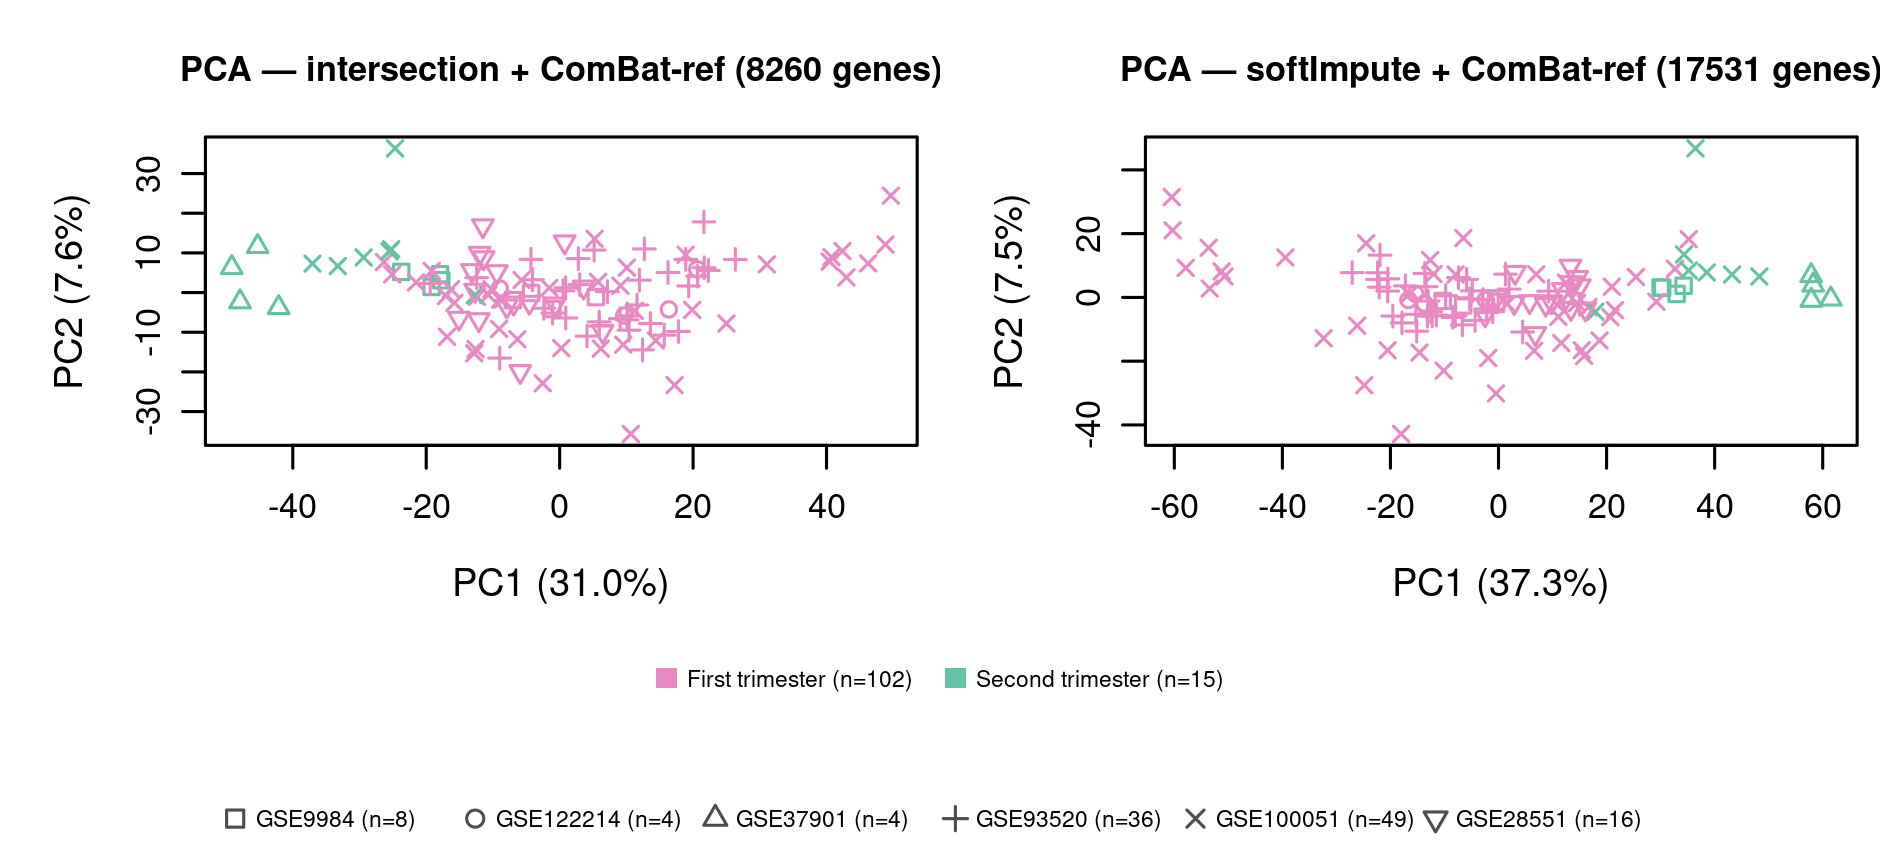
\includegraphics[width=\textwidth]{figures/fig_pca_intersection_softimpute.png}
\caption{PCA of batch-corrected expression matrices after
  reference-batch ComBat (ref = GSE100051). \textbf{Left:}
  intersection-only (8{,}260 genes, no imputation).
  \textbf{Right:} \textit{softImpute}-completed (17{,}531
  genes). Color indicates trimester (pink = first, green =
  second); shape indicates dataset. In both panels, PC1
  separates the two trimesters, confirming that ComBat-ref
  removes batch effects without collapsing the biological
  contrast. The softImpute panel includes 9{,}271 additional
  genes recovered by imputation.}
\label{fig:supp-pca}
\end{figure}

To verify that adding 9{,}271 imputed genes to the ComBat
input does not distort the batch correction of the 8{,}260
genes shared with the intersection-only pipeline, we compared
the post-ComBat-ref corrected expression values for these
shared genes between the two runs. Across all $8{,}260 \times
117 = 966{,}420$ cells, the Pearson correlation was $r =
0.9994$, the mean absolute difference was $0.031$ log$_2$
units ($\sim\!1\%$ of the expression standard deviation),
and the median per-gene MAE was $0.027$.
The genes most affected by the introduction of imputation are
those with the highest within-dataset inter-individual
variability: \textit{HBE1} (within-batch SD $= 3.18$
log$_2$), \textit{SPP1} ($2.79$), \textit{HBG2} ($2.60$),
\textit{CCK} ($2.09$), and \textit{F13A1} ($3.10$) ---
ranks 1--4 and 8 among all 8{,}260 shared genes. Even so, these
worst-case genes have per-gene MAEs of only $0.16$--$0.33$
log$_2$ units (Figure~\ref{fig:supp-combat-sensitivity}), confirming
that adding imputed genes to the ComBat model does not
meaningfully alter the batch-correction estimates for genes
that were already observed.

\begin{figure}[htbp]
\centering
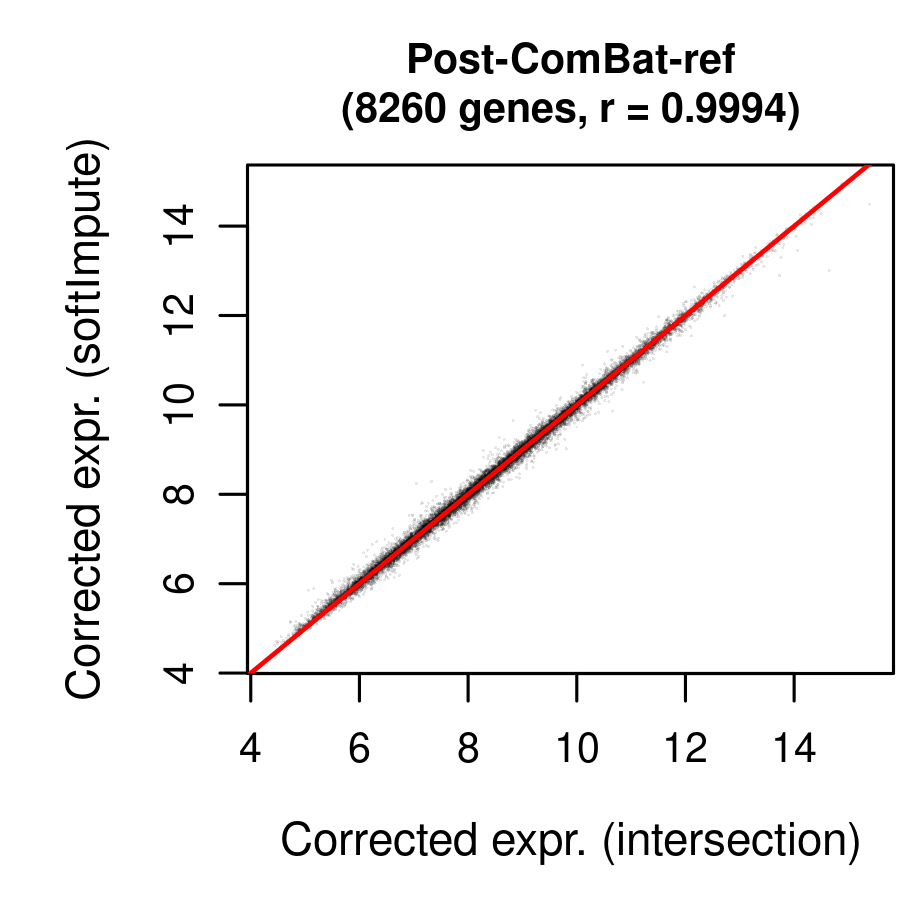
\includegraphics[width=0.49\textwidth]{figures/fig_combat_post_scatter.png}
\hfill
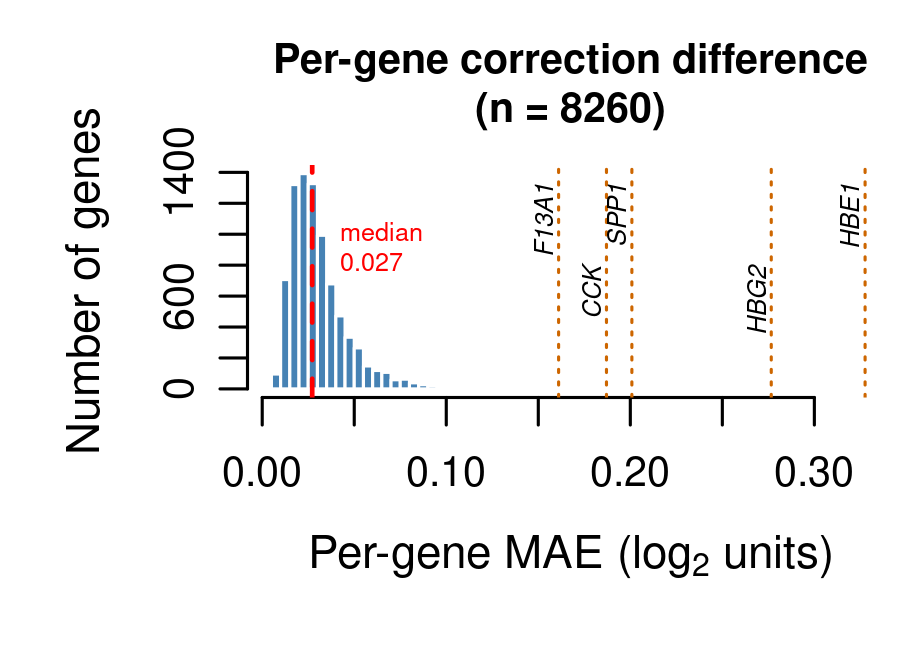
\includegraphics[width=0.49\textwidth]{figures/fig_combat_gene_mae.png}
\caption{ComBat sensitivity analysis: comparison of
  post-ComBat-ref corrected expression for 8{,}260 shared genes
  between the intersection-only and \textit{softImpute}
  pipelines. \textbf{Left:} scatter of corrected values ($r =
  0.9994$ for the 50{,}000 randomly sampled cells shown and
  across all 966{,}420 cells).
  \textbf{Right:} histogram of per-gene mean absolute
  difference; median MAE $= 0.027$ log$_2$ units (dashed
  line; the cell-level \emph{mean} absolute difference is
  $0.031$).}
\label{fig:supp-combat-sensitivity}
\end{figure}

%% -----------------------------------------------------------------
\section{Subsampling validation}
\label{sec:supp-validation}
%% -----------------------------------------------------------------

The DEG list survives resampling of the samples: effect sizes
agree with the full-cohort run at CCC~$= 0.89$ even when the
first-trimester group is cut to ten samples, each random half of
the cohort recovers a median $86.4\%$ of the full-cohort DEGs, and a
balanced two-dataset reference reproduces $86.5\%$ of them. With
the trimester labels shuffled, the same pipeline calls a median
of zero DEGs. The
tests establishing this were run on the first- vs second-trimester comparison (6 datasets, 102
first-trimester $+$ 15 second-trimester $=$ 117 healthy
placental samples; reference: 541~DEGs at FDR${}<0.05$,
$|\text{logFC}|>1$). All tests reused the reference run's
imputed matrix to eliminate \textit{softImpute} stochasticity and
isolate the effect of sample
composition. Because that matrix was fitted on all 117 samples,
each subset's imputed cells carry information from samples the
subset excludes; the stability estimates are therefore
optimistic, and imputation-stage instability is not captured by
these tests.

\paragraph{Sample-size convergence.}
All 15 second-trimester samples were
retained
and the
first-trimester group was subsampled at sizes
$N \in \{10, 16, 20, 25, 30, 40, 50, 60, 80, 100\}$
(30~iterations per size). Three key findings emerged
(Figure~\ref{fig:supp-convergence}):

\begin{enumerate}
  \item \textbf{Effect sizes are stable.} The median (over
    30~iterations) of Lin's concordance correlation coefficient
    (CCC) \citep{Lin1989} --- which, unlike Pearson~$r$, also
    penalizes shifts in location or scale and is therefore the
    stricter test of agreement between effect-size estimates ---
    between subsample and full-cohort log fold-changes was $0.89$
    already at $N\!=\!10$ and rose monotonically to $1.00$ at
    $N\!=\!100$ (Figure~\ref{fig:supp-ccc}).
  \item \textbf{DEG list overlap converges gradually.} Median
    Jaccard index against the full-cohort run rose from $0.54$ at
    $N\!=\!10$ to $0.98$ at $N\!=\!100$
    (Figure~\ref{fig:supp-convergence}, left panel).
  \item \textbf{Retention of reference DEGs is high.}
    At $N\!=\!10$, subsamples retained a median of $90.9\%$ of
    the 541 reference DEGs, rising to $93.0\%$ at $N\!=\!30$
    (Figure~\ref{fig:supp-retention}, first panel). The apparent
    Jaccard drop at small sizes is primarily driven by novel
    DEGs entering the subsample list (genes with noisy
    effect-size estimates that stochastically cross the
    $|\text{logFC}|\!>\!1$ threshold), not by loss of true
    positives. Applying the $|\text{logFC}|$ threshold substantially
    improves stability: FDR-only retention was only $\sim\!59\%$ at
    $N\!=\!10$ (Figure~\ref{fig:supp-retention}, third panel), confirming
    that the threshold selects the reproducible core of genes with
    large, consistent effect sizes.
\end{enumerate}

\paragraph{Label-permutation null.}
Stability does not by itself show that the list is more than
noise: a pipeline artefact would be reproduced in every subset
too. The trimester labels were therefore shuffled across all 117
samples, keeping the group sizes (102 first $+$ 15 second
trimester); each sample's gestational age, which enters ComBat as
the biological covariate, moved with its label, and fetal sex,
dataset membership, the gene set and the imputed matrix were
unchanged. Batch correction and differential expression were then
re-run (200~permutations). With the combined threshold the shuffled
runs called a median of $0$~DEGs (95th percentile~$2$,
maximum~$51$; 166 of 200 runs called none), against 541 for the
real labels; no permutation reached 541 (empirical
$p = 1/201 \approx 0.005$, the smallest attainable with 200
permutations; Figure~\ref{fig:supp-permutation}, left). The
shuffled DEGs were not the real ones: a median of 0 (maximum~39)
overlapped the 541.

By FDR alone the null was not empty. A median of 216 genes
(95th percentile~$729$, maximum~$2{,}280$) reached FDR${}<0.05$,
against 7{,}779 in the real run
(Figure~\ref{fig:supp-permutation}, right), and a median of
258~genes had $p<0.001$, where about 18 are expected under the
null. This is not leakage of real signal through the shuffled
labels: runs in which no true second-trimester sample landed in
the ``second-trimester'' group showed the same inflation. When
ComBat was skipped and dataset entered the \textit{limma} design
instead (50~permutations), the inflation disappeared (median
13.5~genes at $p<0.001$, 0 at FDR${}<0.05$). The excess therefore
comes from ComBat: with datasets that hold only one trimester,
batch-effect estimates absorb part of the group contrast, and the
corrected data then carry less variance than \textit{limma}
assumes \citep{Nygaard2016}. The $|\text{logFC}|>1$ cutoff
removes these small spurious effects; this is a further reason
to report the combined threshold rather than FDR alone.

\paragraph{Split-half reproducibility.}
Following the multiple random validation strategy introduced by
\citet{Michiels2005}, the full sample was randomly split into two
halves maintaining the trimester ratio (50~iterations). Median
Jaccard between halves was $0.453$, reflecting the limited
statistical power of 7--8 second-trimester samples per half.
However, each half retained a median of $86.4\%$ of the full-cohort
DEGs (Figure~\ref{fig:supp-split-half}, bottom left), and log
fold-change CCC between halves was $0.771$
(Figure~\ref{fig:supp-split-half}, top right). The split-half
Jaccard of $0.45$ is typical for microarray studies with small
contrast groups \citep{EinDor2006} and does not indicate fragility
of the core result.

\paragraph{Robustness to design imbalance.}
To test whether the design imbalance --- some datasets
contribute samples from only one trimester, which can bias
ComBat batch-effect estimates --- inflates the DEG
list, we compared against a balanced 2-dataset
reference
(GSE100051 $+$ GSE9984; 46 first-trimester $+$ 11
second-trimester samples; ComBat; 484~DEGs). Of the
541 full-integration DEGs, $86.5\%$ ($468/541$) also appeared in
the balanced reference (Jaccard $= 0.840$); conversely
$96.7\%$ ($468/484$) of the balanced reference's DEGs are
retained, and log fold-change agreement over
the union of the two DEG lists is CCC~$= 0.99$ (Figure~\ref{fig:supp-ccc}, right panel).
The 73 full-integration DEGs absent from the balanced reference
list are threshold effects, not fabricated signal: all 73 show
the same direction of change in the balanced run, 62 are already
FDR-significant there and miss only the $|\text{logFC}| > 1$
cutoff (median balanced $|\text{logFC}| = 0.96$; 72 of 73 exceed
$0.8$), and only 3 fail both criteria, none with discordant
direction. Conversely, all 16 balanced-reference DEGs absent
from the full-cohort list agree in direction with the full-cohort run.
Even at $N\!=\!10$, subsamples retained $\sim\!93\%$ of the
balanced reference DEGs (Figure~\ref{fig:supp-retention}, second
panel). Across the whole size range the subsamples recover this
independent reference at nearly the same rate as they recover
the full-cohort run's own DEG list --- the two retention curves differ
by at most $0.052$ at any size
(Figure~\ref{fig:supp-convergence}, right panel).

\begin{figure}[htbp]
\centering
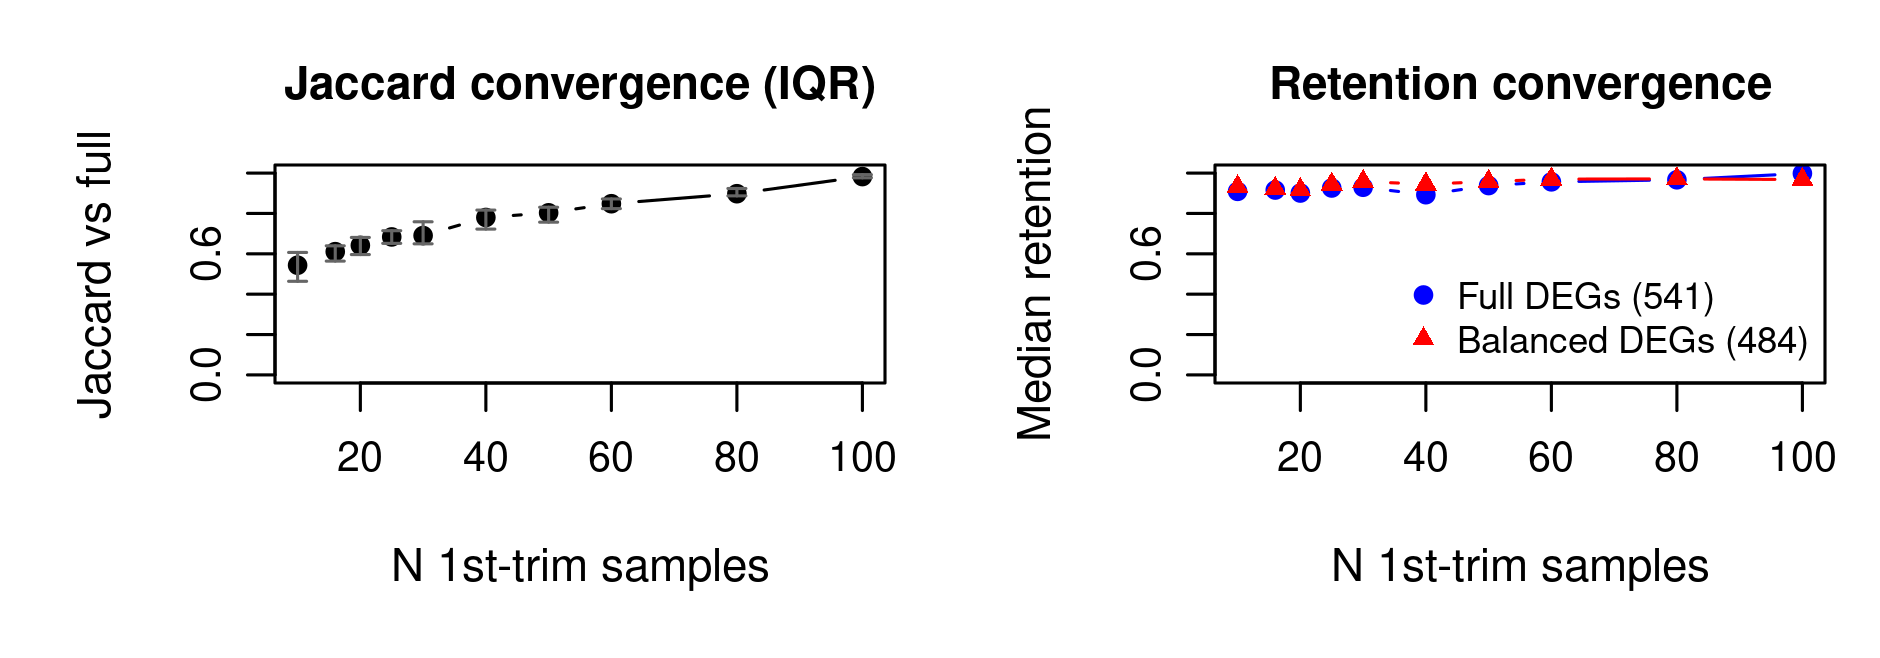
\includegraphics[width=\textwidth]{figures/fig_validation_convergence.png}
\caption{Subsampling validation summary. \textbf{Left:}
  Jaccard index of DEG lists versus the full-cohort reference
  as a function of first-trimester sample size (median with
  IQR). \textbf{Right:} median retention, by the \emph{same}
  subsampled runs, of two reference DEG lists: blue --- the
  541~DEGs of the full integration; red --- the 484~DEGs of
  the balanced 2-dataset reference, which is fitted once on
  all of its samples and is itself never subsampled.}
\label{fig:supp-convergence}
\end{figure}

\begin{figure}[htbp]
\centering
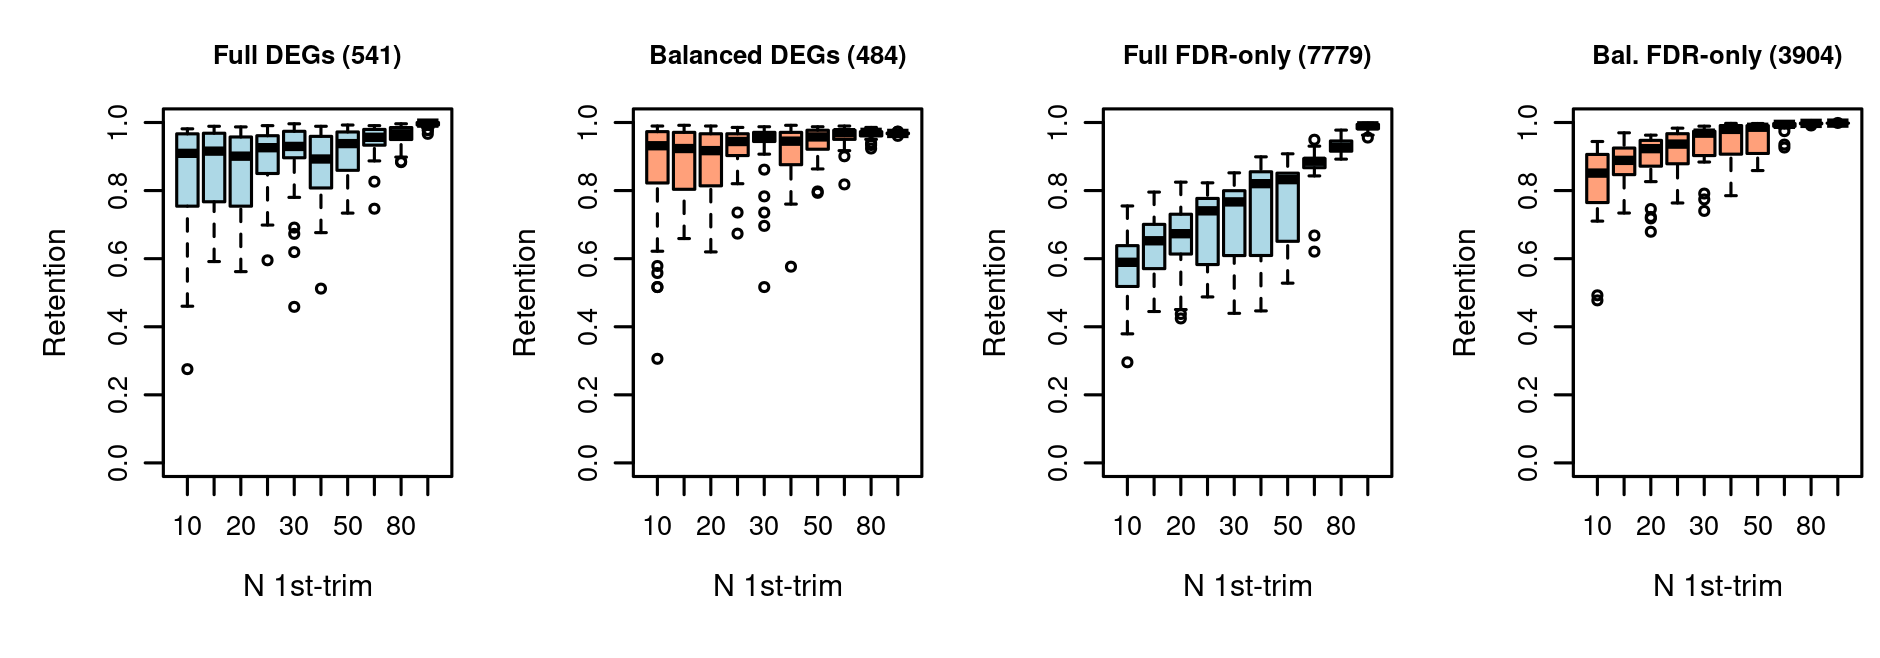
\includegraphics[width=\textwidth]{figures/fig_validation_retention.png}
\caption{Retention of reference DEGs across subsampling sizes.
  Each panel shows the fraction of a given reference set's DEGs
  that appear in the subsample's DEG list. From left to right:
  full-cohort DEGs (FDR$+$logFC, 541~genes); balanced-reference
  DEGs (FDR$+$logFC, 484~genes); full-cohort FDR-only DEGs
  (7{,}779~genes); balanced-reference FDR-only DEGs
  (3{,}904~genes).}
\label{fig:supp-retention}
\end{figure}

\begin{figure}[htbp]
\centering
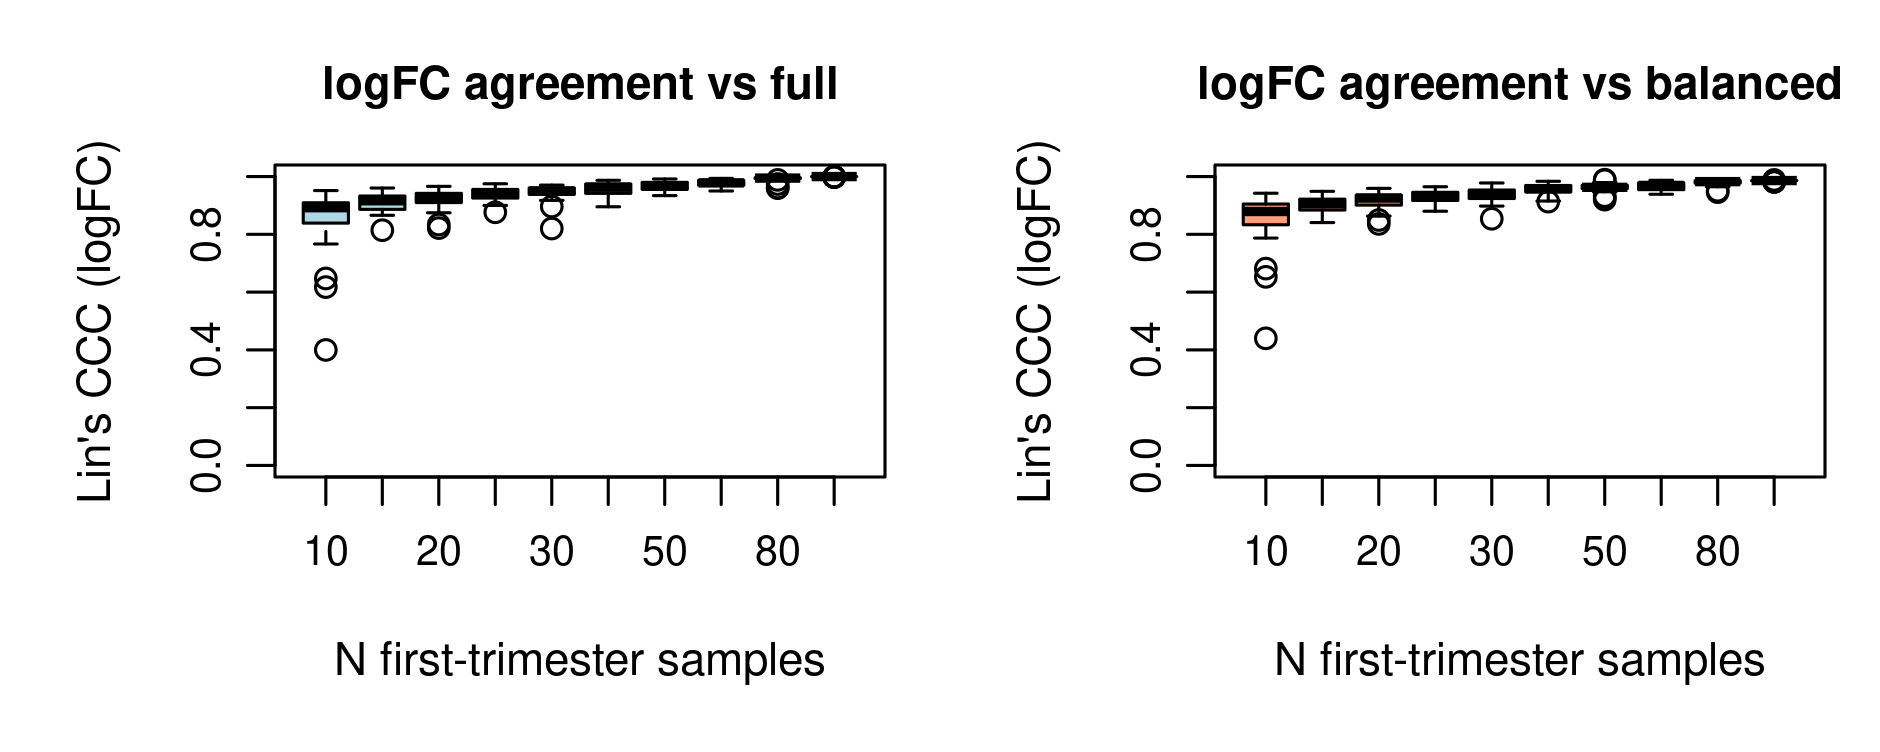
\includegraphics[width=\textwidth]{figures/fig_validation_ccc.png}
\caption{Log fold-change agreement (Lin's concordance
  correlation coefficient) between subsampled and reference
  runs. \textbf{Left:} versus the full 6-dataset integration.
  \textbf{Right:} versus the balanced 2-dataset reference.
  CCC~$= 1$ only when log fold-changes are numerically
  identical.}
\label{fig:supp-ccc}
\end{figure}

\begin{figure}[htbp]
\centering
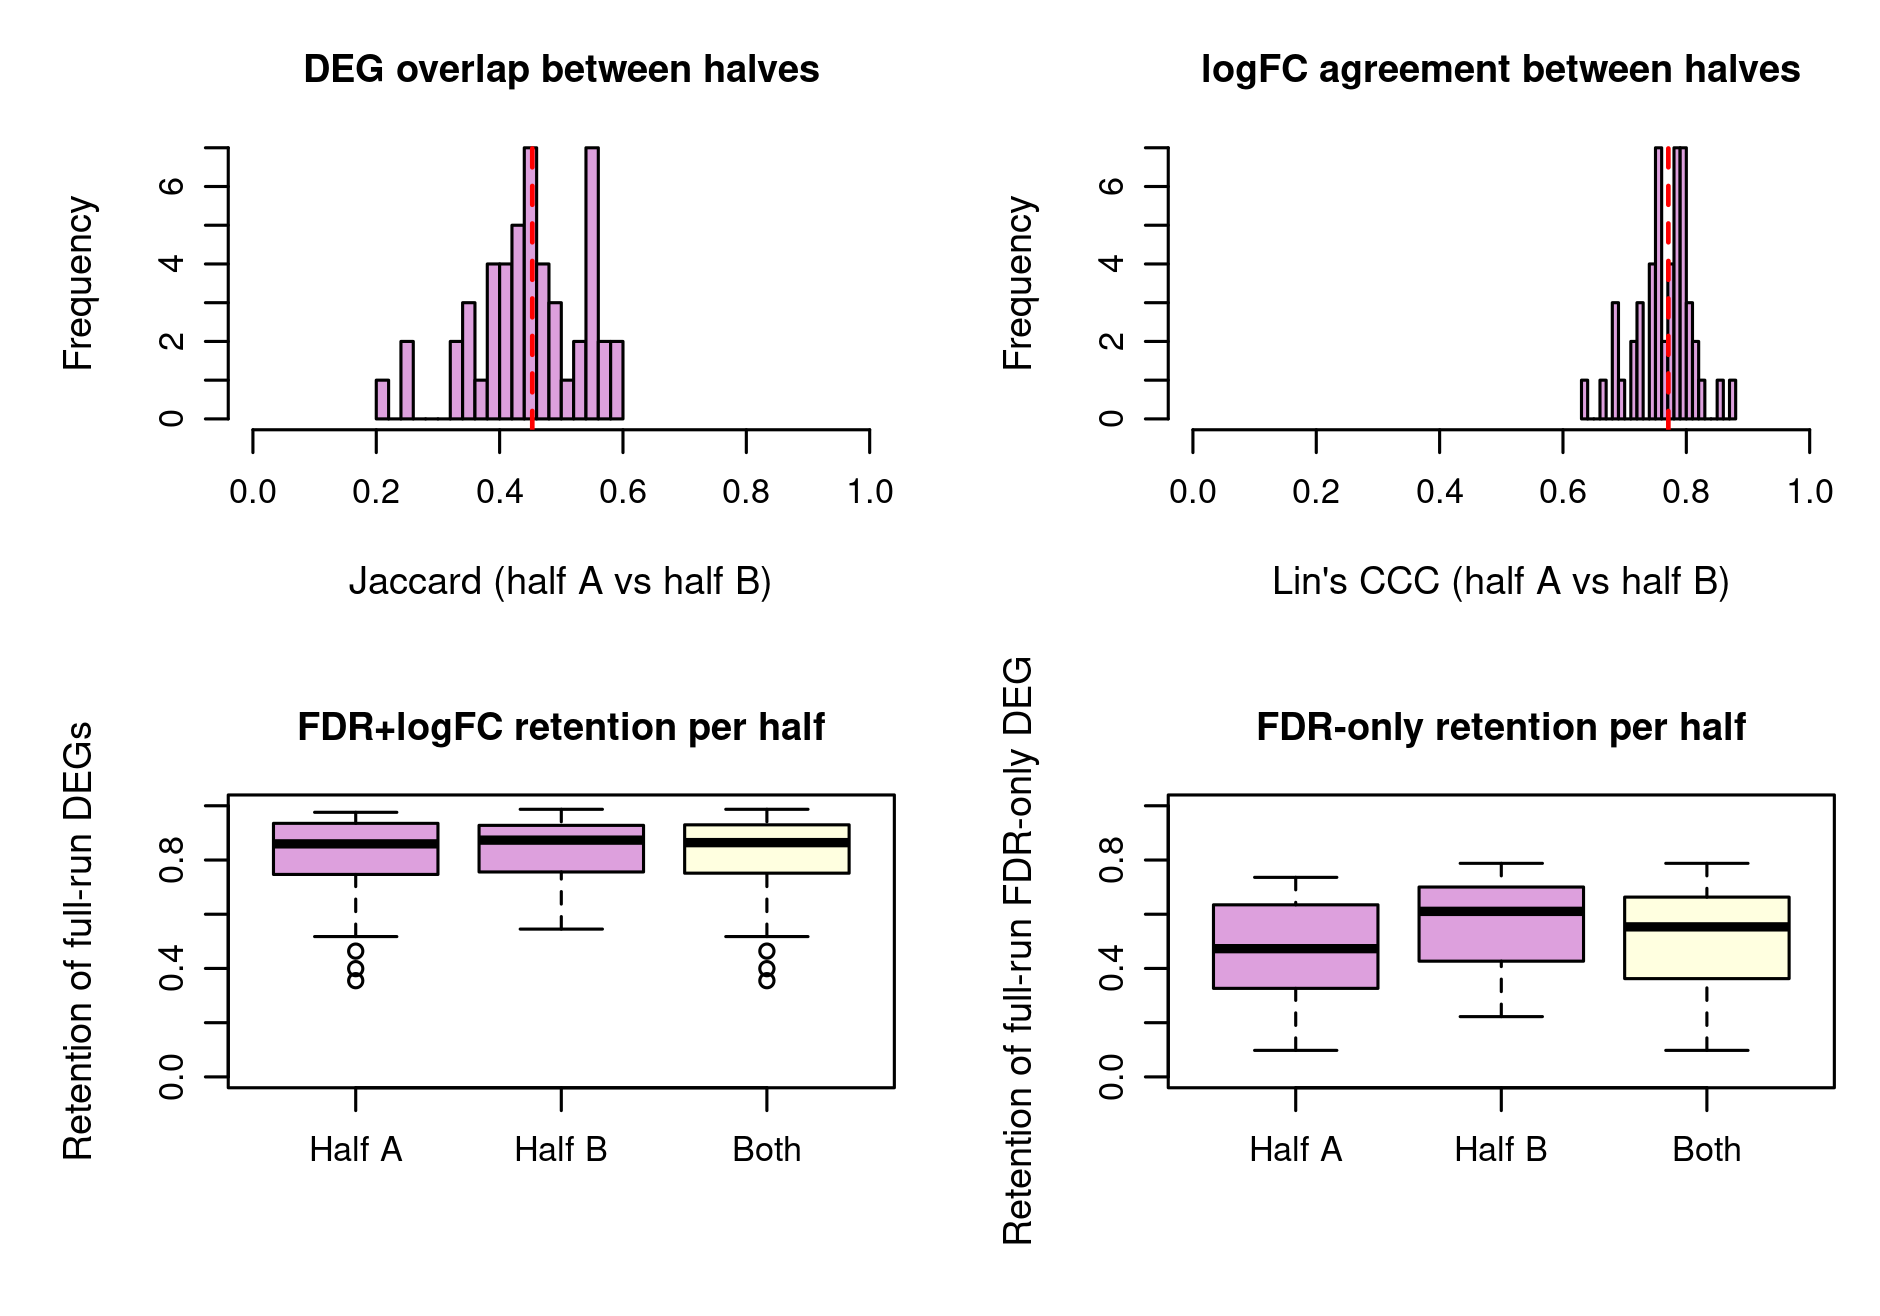
\includegraphics[width=\textwidth]{figures/fig_validation_split_half.png}
\caption{Stratified split-half validation (50~iterations).
  \textbf{Top left:} Jaccard between halves' DEG lists.
  \textbf{Top right:} Lin's CCC of log fold-changes between
  halves. \textbf{Bottom left:} retention of full-cohort DEGs
  (FDR$+$logFC) per half. \textbf{Bottom right:} retention of
  full-cohort FDR-only DEGs per half.}
\label{fig:supp-split-half}
\end{figure}

\begin{figure}[htbp]
\centering
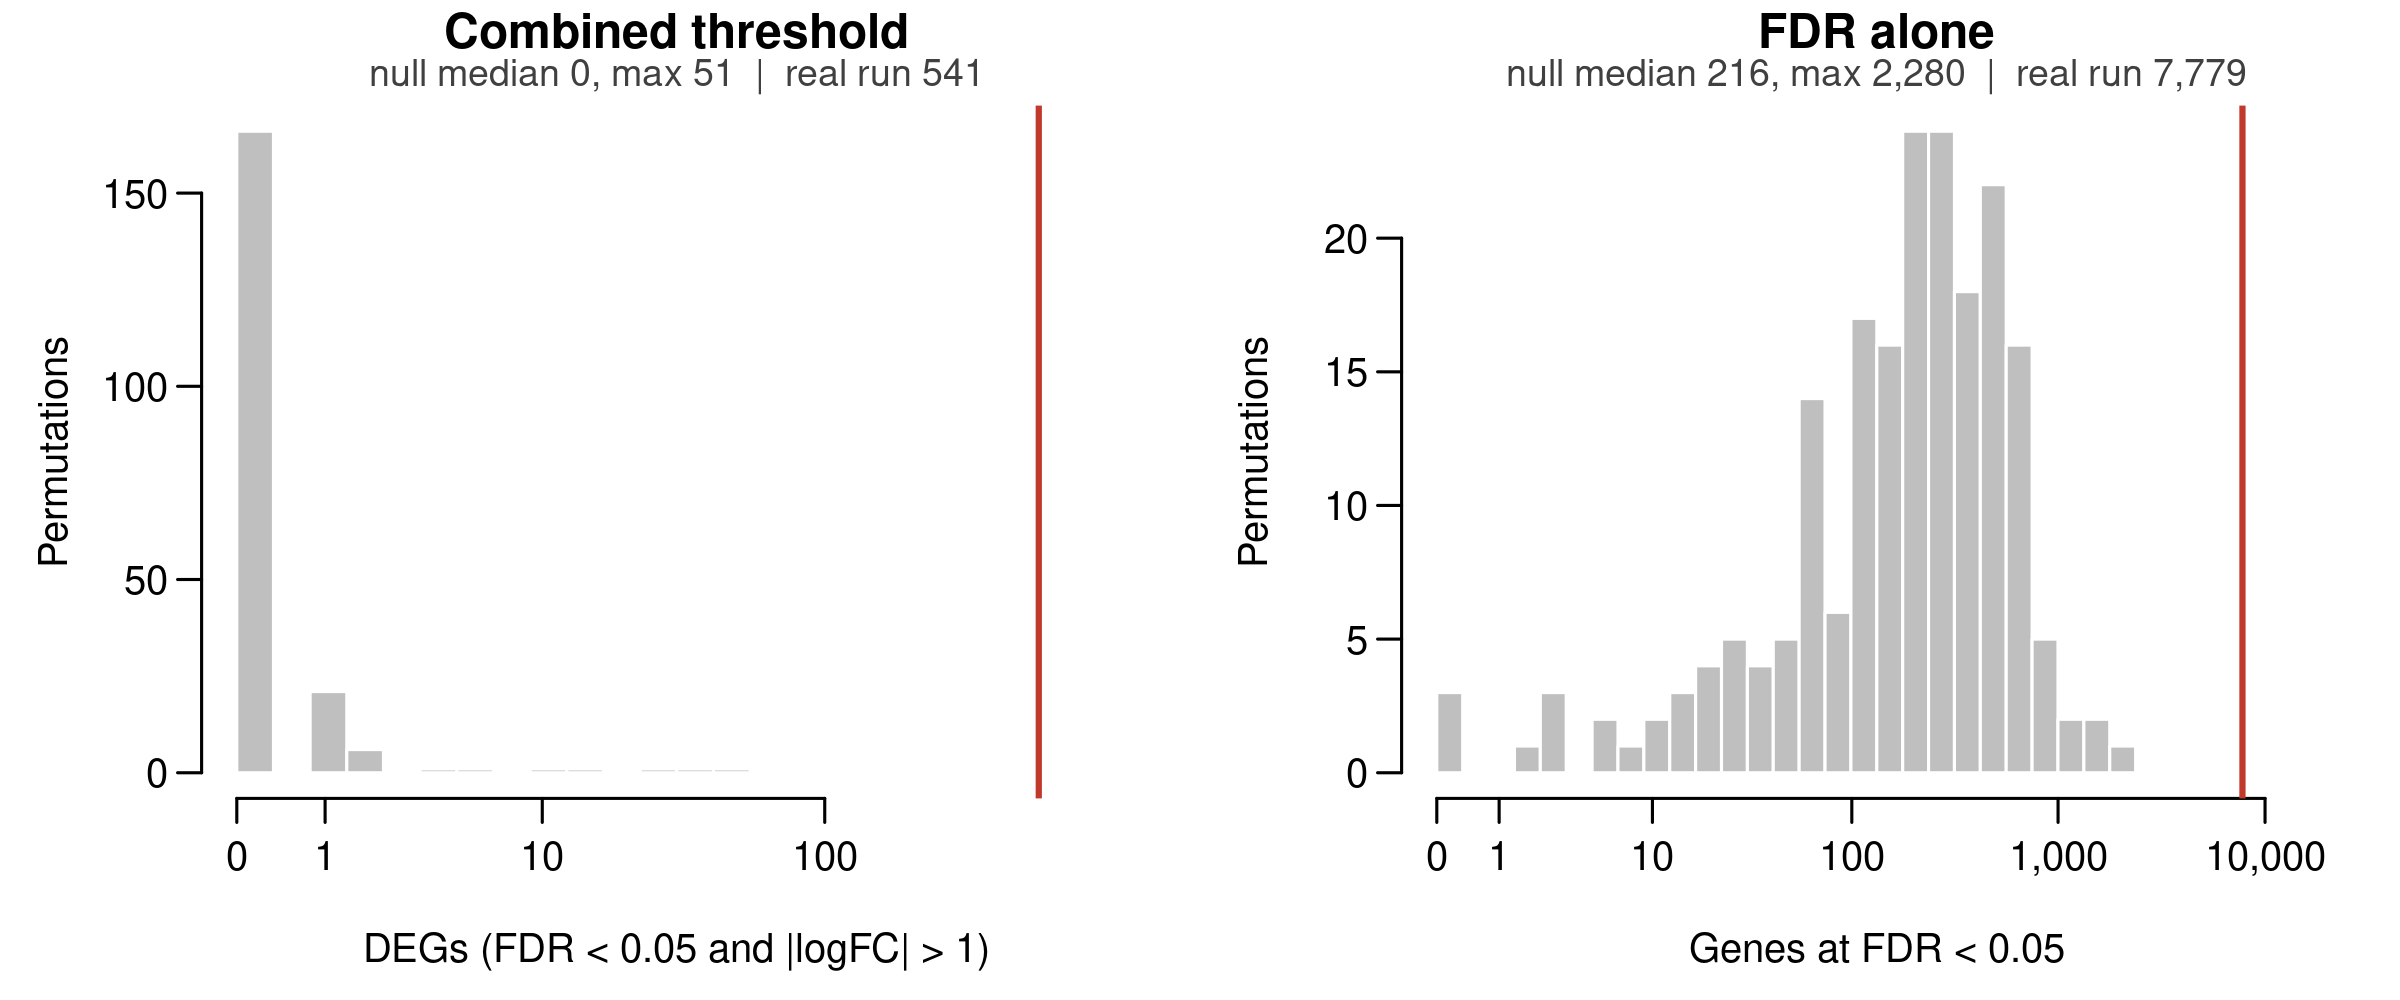
\includegraphics[width=\textwidth]{figures/fig_validation_permutation.png}
\caption{Label-permutation null (200 permutations of the
  trimester labels, with gestational age moved alongside).
  Histograms of the number of genes called per shuffled run
  (log scale); red line --- the real run. \textbf{Left:}
  combined threshold (FDR${}<0.05$ and $|\text{logFC}|>1$).
  \textbf{Right:} FDR${}<0.05$ alone.}
\label{fig:supp-permutation}
\end{figure}

%% -----------------------------------------------------------------
\section{Concordance with prior single-platform integrative analysis}
\label{sec:supp-concordance}
%% -----------------------------------------------------------------

The 2021 analysis is not independent of the present one: 16 of
its 22 samples (GSE9984, GSE37901, GSE122214) are included in
this cohort, so the comparison below is a consistency check
across processing strategies rather than external
corroboration. Of the 265 gained DEGs, 245 (92.5\%) were
present in the Lykhenko 2021 protein-coding limma table. The remaining 20 are on genes
absent from Affymetrix platforms and therefore had no prior
estimate to compare against; they include an immune/defensin
cluster (\textit{DEFA1}, \textit{DEFA1B}, \textit{DEFA3},
\textit{CCL3}, \textit{CCL3L3}, \textit{FCGR1A},
\textit{FCGR2A}), two chorionic gonadotropin $\beta$-subunit
genes (\textit{CGB2}, \textit{CGB7}), and eleven other genes
with no obvious functional grouping. Among the 245 matched genes,
218 (89.0\%) showed the same direction of change, and 149
(60.8\%) were already significant at $\text{FDR} < 0.05$ in the
2021 analysis --- lost only because the cross-platform intersection
step discarded them when non-Affymetrix platforms were added. The
concordance of log fold-changes between the two analyses was
CCC~$= 0.43$ for the gained genes (Pearson $r = 0.61$; the 2021
effect sizes are systematically smaller, mean $|\text{logFC}|$
$0.59$ against $1.41$ here). 27 genes (11.0\%)
showed opposite direction --- a non-negligible fraction, but
one whose composition rules out systematic bias: none of the
27 was significant in the 2021 analysis
($\text{FDR} < 0.05$: 0/27), their 2021 effect sizes are
noise-level (median $|\text{logFC}| = 0.13$, versus $0.56$
for the direction-concordant genes), and all 149 matched genes
that \emph{were} significant in 2021 agree in direction
(149/149). The disagreements are thus confined to genes where
the prior analysis had no signal to disagree with.

For the 8{,}260 genes shared between the softImpute and
intersection-only analyses, the internal log fold-change
correlation was near-perfect ($r = 0.9988$), with 98\% of
genes retaining the same direction and only 29 genes called
significant by one analysis alone (28 by softImpute, one by
intersection), all of them $|\text{logFC}|$-threshold effects. This confirms that imputation preserves the
effect-size landscape of the originally observed
genes.

%% -----------------------------------------------------------------
\section{Holdout validation of differential expression on imputed genes}
\label{sec:supp-blockholdout}
%% -----------------------------------------------------------------

Masking real measurements and re-running the whole pipeline
shows that it is conservative rather than credulous: under
every masking scheme fewer than $0.15\%$ of masked non-DEGs are
newly called, while $8$--$67\%$ of true DEGs are lost. What
decides the loss is not how much coverage a gene keeps but
whether it keeps a real measurement in the ComBat reference
batch --- under gene--dataset block masking, $7.0\%$ of true
DEGs are lost when it does and $96.8\%$ when it does not.

Neither Section~\ref{sec:supp-imputation} (accuracy of the
imputed \emph{values}) nor Section~\ref{sec:supp-validation}
(stability under resampling of \emph{samples}) answers that
question, which is the one that matters for the 265 gained
genes: when a gene is called differentially expressed from a
matrix in which most of its cells were imputed and every cell
was then batch-corrected, is the call correct? The experiment
below supplies a known answer, on exactly the masks of
Section~\ref{sec:supp-imputation}, so that the accuracy of the
values and the accuracy of the calls refer to the same masked
cells. The main text (Section~``Holdout validation of
differential expression on imputed genes'') reports the
gene--dataset block scheme; this section gives all three
schemes, both ComBat variants, seven imputers, the
Reference/Masked/Oracle comparison and a repeat with imputed cells
at full weight.

\paragraph{Design.}
For each masking scheme and repeat, the masked matrix that each
imputer filled in Section~\ref{sec:supp-imputation} was carried
through the rest of the pipeline --- reference-batch ComBat with
the production covariates, then \textit{limma} with weight~0 on
every masked and every originally-missing cell --- and its DEG
calls compared with the same imputer's run on the unmasked
matrix. Three runs are compared:

\smallskip
\noindent
\begin{tabularx}{\textwidth}{@{}lXX@{}}
\toprule
\textbf{Run} & \textbf{How it is built} &
  \textbf{What its comparison isolates} \\
\midrule
\textbf{Reference} & Nothing masked. For \textit{softImpute} this is
  the primary analysis and returns its 541 DEGs. &
  The known answer, against which the other two are scored. \\
\addlinespace
\textbf{Masked} & Masked cells imputed, ComBat fitted on the
  partially imputed matrix, \textit{limma} with weight~0 on
  every filled cell. This is the production treatment. &
  \textbf{Masked} vs \textbf{Reference}: everything masking costs,
  end to end. \\
\addlinespace
\textbf{Oracle} & The same surviving measurements and weights
  as \textbf{Masked}, but corrected with the reference run's
  ComBat parameters. &
  \textbf{Oracle} vs \textbf{Reference}: the loss of real samples
  alone. \textbf{Masked} vs \textbf{Oracle}: the distortion
  transmitted through the batch-correction pathway. \\
\bottomrule
\end{tabularx}
\smallskip

\noindent
Genes that masking leaves
without a real measurement in one trimester are dropped before
testing, as the production pipeline drops them, and are counted
as lost. A gene can be masked in more than one repeat:
Table~\ref{tab:supp-confusion} reports counts per repeat, as
mean $\pm$ SD over the three seeded repeats, so they are on
the scale of one run, while Tables~\ref{tab:supp-arms}
and~\ref{tab:supp-blockholdout} pool gene-level results over
the repeats, where one gene contributes up to three of them. One stratum needs
reading with care: under random-cell masking no gene loses a
whole block, so ``GSE100051 masked'' there is not a masking
effect at all but simply the 5{,}770 genes with no GSE100051
measurement in the real data; it contains no true DEG, because
none of the gained DEGs lacks the reference batch.
Two variants of the design were run for \textit{softImpute} on
the same masks and imputations: plain ComBat (no reference
batch; its own reference run gives 508 DEGs) and imputed cells at
weight~1 instead of~0.

\begin{table}[htbp]
\centering
\footnotesize
\begingroup\setlength{\tabcolsep}{3pt}
\begin{tabular}{@{}lrrrrrrr@{}}
\toprule
\textbf{Stratum} & \textbf{Genes} & \textbf{Stayed DEG} & \textbf{DEG $\to$ not} & \textbf{Not $\to$ DEG} & \textbf{Stayed not} & \textbf{Lost \%} & \textbf{Gained \%} \\
\midrule
\multicolumn{8}{@{}l}{\textit{random cells} (17{,}531 genes per run; 0 dropped before testing)} \\[2pt]
all masked genes & 17{,}531 & 500 $\pm$ 4 & 41 $\pm$ 4 & 22 $\pm$ 2 & 16968 $\pm$ 2 & 7.6 & 0.13 \\
GSE100051 kept & 11{,}761 & 500 $\pm$ 4 & 41 $\pm$ 4 & 22 $\pm$ 2 & 11198 $\pm$ 2 & 7.6 & 0.19 \\
GSE100051 masked & 5{,}770 & 0 $\pm$ 0 & 0 $\pm$ 0 & 0 $\pm$ 0 & 5770 $\pm$ 0 & -- & 0.00 \\
\addlinespace
\multicolumn{8}{@{}l}{\textit{gene--dataset block} (5{,}157 genes per run; 28 dropped before testing)} \\[2pt]
all masked genes & 5{,}157 & 140 $\pm$ 12 & 51 $\pm$ 9 & 7 $\pm$ 2 & 4960 $\pm$ 60 & 26.6 & 0.13 \\
GSE100051 kept & 3{,}911 & 138 $\pm$ 12 & 10 $\pm$ 2 & 7 $\pm$ 2 & 3756 $\pm$ 61 & 7.0 & 0.18 \\
GSE100051 masked & 1{,}246 & 1 $\pm$ 1 & 40 $\pm$ 8 & 0 $\pm$ 0 & 1204 $\pm$ 7 & 96.8 & 0.00 \\
\addlinespace
\multicolumn{8}{@{}l}{\textit{worst-case block} (2{,}815 genes per run; 407 dropped before testing)} \\[2pt]
all masked genes & 2{,}815 & 30 $\pm$ 9 & 60 $\pm$ 12 & 4 $\pm$ 2 & 2721 $\pm$ 20 & 66.7 & 0.13 \\
GSE100051 kept & 690 & 30 $\pm$ 9 & 3 $\pm$ 2 & 4 $\pm$ 2 & 654 $\pm$ 25 & 9.1 & 0.56 \\
GSE100051 masked & 2{,}125 & 0 $\pm$ 0 & 57 $\pm$ 10 & 0 $\pm$ 0 & 2068 $\pm$ 14 & 100.0 & 0.00 \\
\bottomrule
\end{tabular}
\endgroup
\caption{DEG calls after masking versus the reference run,
  \textit{softImpute} $+$ ComBat-ref, by masking scheme and by
  whether the gene retains a real measurement in GSE100051 (the
  largest dataset and the ComBat reference batch). Counts are
  genes per run, mean $\pm$ SD over three repeats; dropped genes
  are counted under ``DEG $\to$ not'' / ``stayed not'' according
  to their reference-run status. ``Lost \%'': true DEGs no longer
  called; ``Gained \%'': true non-DEGs newly called, both from the
  per-run means. Pooled over repeats and with their standard
  deviations, the same quantities are the \textbf{Sens.\ M} and
  \textbf{Spec.\ M} columns of Table~\ref{tab:supp-arms}.}
\label{tab:supp-confusion}
\end{table}

\paragraph{Result: conservative, not credulous.}
Under every scheme the number of genes that newly cross the DEG
threshold is tiny --- $0.13\%$ of the masked non-DEGs under
each of the three schemes for random cells, gene--dataset block and
worst-case masking (the complement of \textbf{Spec.\ M} in
Table~\ref{tab:supp-arms}; the counts themselves are in
Table~\ref{tab:supp-confusion}) --- and is
zero precisely where the damage to detection is greatest, when
GSE100051 is masked.
Masking removes DEGs; it does not create them. How many it
removes depends on what is masked: $7.6\%$ of true DEGs
under random cells (the $|\text{logFC}| = 1$ threshold-crossing
noise floor), $26.6\%$ under gene--dataset block masking and
$66.7\%$ under the worst-case mask; and within the block
scheme $7.0\%$ when the gene keeps its GSE100051 block against
$96.8\%$ when it does not, with the median fold-change of the
true DEGs shrinking to $0.28$ of its reference-run value in the latter
stratum ($0.09$ under the worst-case mask).

\begin{table}[htbp]
\centering
\footnotesize
\begingroup\setlength{\tabcolsep}{3pt}
\begin{tabular}{@{}lrrrrrr@{}}
\toprule
\textbf{Masked dataset (1st/2nd)} & \textbf{True DEGs} & \textbf{Lost} & \textbf{Gained} & \textbf{Lost \%} & \textbf{$|$logFC$|$ ratio} & \textbf{Oracle sens.\ \%} \\
\midrule
\multicolumn{7}{@{}l}{\textit{ComBat-ref}} \\[2pt]
GSE100051 (42/7) & 20 $\pm$ 2 & 19 $\pm$ 3 & 0 $\pm$ 0 & 94.6 & 0.33 & 95.0 \\
GSE37901 (0/4) & 22 $\pm$ 5 & 4 $\pm$ 1 & 0 $\pm$ 0 & 17.8 & 0.89 & 82.2 \\
GSE93520 (36/0) & 21 $\pm$ 7 & 2 $\pm$ 1 & 0 $\pm$ 0 & 11.2 & 0.95 & 92.7 \\
GSE9984 (4/4) & 20 $\pm$ 1 & 1 $\pm$ 1 & 2 $\pm$ 1 & 3.5 & 1.03 & 100.0 \\
GSE122214 (4/0) & 24 $\pm$ 6 & 0 $\pm$ 0 & 0 $\pm$ 0 & 0.0 & 1.00 & 100.0 \\
GSE28551 (16/0) & 21 $\pm$ 6 & 0 $\pm$ 0 & 2 $\pm$ 2 & 0.0 & 1.06 & 100.0 \\
\addlinespace
\multicolumn{7}{@{}l}{\textit{plain ComBat}} \\[2pt]
GSE100051 (42/7) & 20 $\pm$ 2 & 19 $\pm$ 3 & 0 $\pm$ 0 & 93.1 & 0.38 & 93.5 \\
GSE37901 (0/4) & 21 $\pm$ 4 & 4 $\pm$ 2 & 0 $\pm$ 0 & 18.2 & 0.88 & 81.8 \\
GSE93520 (36/0) & 21 $\pm$ 7 & 2 $\pm$ 2 & 0 $\pm$ 0 & 9.8 & 0.94 & 94.3 \\
GSE9984 (4/4) & 20 $\pm$ 2 & 1 $\pm$ 1 & 3 $\pm$ 1 & 3.3 & 1.06 & 100.0 \\
GSE122214 (4/0) & 21 $\pm$ 6 & 0 $\pm$ 1 & 0 $\pm$ 0 & 1.3 & 1.00 & 98.7 \\
GSE28551 (16/0) & 19 $\pm$ 7 & 0 $\pm$ 0 & 3 $\pm$ 1 & 0.0 & 1.06 & 100.0 \\
\bottomrule
\end{tabular}
\endgroup
\caption{Gene--dataset block masking, genes with exactly one
  dataset masked, split by that dataset (first/second-trimester
  samples in parentheses), for \textit{softImpute} with
  reference-batch ComBat and with plain ComBat on the same masks
  and imputations; each variant is compared with its own full
  run. Mean $\pm$ SD over three repeats, per run. ``$|$logFC$|$
  ratio'': median masked/reference fold-change among true DEGs;
  ``Oracle sens.'': share of true DEGs recovered when the same
  surviving measurements are corrected with the reference run's
  parameters.}
\label{tab:supp-bydataset}
\end{table}

\paragraph{Which dataset is masked matters, not how much.}
Table~\ref{tab:supp-bydataset} separates the two things
GSE100051 is: the batch holding 49 of the 117 samples and 7 of
the 15 second-trimester samples, and the ComBat reference.
Masking the small second-trimester-only batch GSE37901 costs
$18\%$ of true DEGs but leaves fold-changes essentially intact
(median ratio $0.89$) and \textbf{Masked} indistinguishable from
\textbf{Oracle} --- that is loss of power from 4 of 15
second-trimester samples, and nothing else. Masking GSE100051
costs $95\%$ with fold-changes shrunk to a third ($0.33$), while the
\textbf{Oracle} recovers $95\%$: with the same 7 second-trimester
samples gone, ComBat parameters estimated on real data would
still have found the genes. With plain ComBat the picture is the
same --- GSE100051 masked: $93\%$ lost, ratio $0.38$; GSE37901
masked: $18\%$, ratio $0.88$ --- so the effect is not tied
to reference designation. Both ComBat variants rescale every
batch onto a common location and scale that a 49-sample
synthetic block dominates; because the imputed block carries
the low-rank consensus rather than the gene's real
between-trimester difference, the real measurements are pulled
toward it and true effects fall below the $|\text{logFC}| > 1$
cutoff. Reconstruction quality is not the cause: on these same
genes the per-gene imputation error differs by only about
$0.2$ log$_2$ units between the strata
(Table~\ref{tab:supp-imputation-pergene}). Masking any
first-trimester-only batch costs little --- at most $11\%$, for
the 36-sample GSE93520 --- as expected with 102 first-trimester
samples.
Table~\ref{tab:supp-arms} gives the full three-way
decomposition for \textit{softImpute} under every scheme and
stratum.

\begin{table}[htbp]
\centering
\scriptsize
\begingroup\setlength{\tabcolsep}{2.5pt}
\begin{tabular}{@{}lrrrrrrrrr@{}}
\toprule
\textbf{Stratum} & \textbf{Genes} & \textbf{True} & \multicolumn{4}{c}{\textbf{log fold-change agreement between runs}} & \multicolumn{2}{c}{\textbf{Sens.\ \%}} & \textbf{Spec.\ \%} \\
\cmidrule(lr){4-7}\cmidrule(lr){8-9}
 & & \textbf{DEGs} & \textbf{$r$ M,R} & \textbf{MAE M,R} & \textbf{MAE O,R} & \textbf{MAE M,O} & \textbf{M} & \textbf{O} & \textbf{M} \\
\midrule
\multicolumn{10}{@{}l}{\textit{random cells} (0 dropped before testing)} \\[2pt]
all masked genes & 52{,}593 & 1623 & 0.993 & 0.029 & 0.015 & 0.023 & 92.4\,$\pm$\,0.8 & 96.7\,$\pm$\,0.7 & 99.9\,$\pm$\,0.0 \\
GSE100051 kept & 35{,}283 & 1623 & 0.994 & 0.035 & 0.020 & 0.025 & 92.4\,$\pm$\,0.8 & 96.7\,$\pm$\,0.7 & 99.8\,$\pm$\,0.0 \\
GSE100051 masked & 17{,}310 & 0 & 0.946 & 0.018 & 0.006 & 0.017 & -- & -- & 100.0\,$\pm$\,0.0 \\
\addlinespace
\multicolumn{10}{@{}l}{\textit{gene--dataset block} (84 dropped before testing)} \\[2pt]
all masked genes & 15{,}471 & 571 & 0.928 & 0.072 & 0.036 & 0.058 & 73.4\,$\pm$\,5.2 & 93.3\,$\pm$\,2.2 & 99.9\,$\pm$\,0.0 \\
GSE100051 kept & 11{,}734 & 446 & 0.994 & 0.028 & 0.024 & 0.007 & 93.0\,$\pm$\,1.5 & 94.2\,$\pm$\,1.4 & 99.8\,$\pm$\,0.1 \\
GSE100051 masked & 3{,}737 & 125 & 0.760 & 0.216 & 0.073 & 0.220 & 3.2\,$\pm$\,1.6 & 90.2\,$\pm$\,4.0 & 100.0\,$\pm$\,0.0 \\
\addlinespace
\multicolumn{10}{@{}l}{\textit{worst-case block} (1{,}221 dropped before testing)} \\[2pt]
all masked genes & 8{,}445 & 270 & 0.728 & 0.129 & 0.064 & 0.110 & 33.3\,$\pm$\,11.1 & 84.9\,$\pm$\,3.9 & 99.8\,$\pm$\,0.1 \\
GSE100051 kept & 2{,}071 & 99 & 0.983 & 0.059 & 0.058 & 0.007 & 90.9\,$\pm$\,7.9 & 91.9\,$\pm$\,5.7 & 99.4\,$\pm$\,0.3 \\
GSE100051 masked & 6{,}374 & 171 & 0.471 & 0.157 & 0.067 & 0.151 & 0.0\,$\pm$\,0.0 & 79.7\,$\pm$\,1.6 & 100.0\,$\pm$\,0.0 \\
\bottomrule
\end{tabular}
\endgroup
\caption{Three-way holdout comparison for \textit{softImpute},
  by masking scheme and GSE100051 stratum. \textbf{R}eference,
  \textbf{M}asked and \textbf{O}racle are the three runs
  defined under \emph{Design} above. ``Genes'' is
  the number of gene-level results pooled over three repeats and
  ``True DEGs'' those significant in the reference run. $r$ and MAE
  are the Pearson correlation and mean absolute difference
  between the log fold-changes two runs' \textit{limma} tables
  assign to the same genes.
  Sensitivity is the fraction of true DEGs still called by each
  run, specificity the fraction of true non-DEGs left uncalled
  by the masked run (FDR${}<0.05$, $|\text{logFC}|>1$); the
  point values pool genes across the three repeats, $\pm$ the
  standard deviation of the three per-repeat percentages. ``--'':
  no true DEG in the stratum.}
\label{tab:supp-arms}
\end{table}

Throughout this section $r$ and MAE compare differential
expression estimates --- the log fold-changes two runs assign
to the same gene --- and not the imputed values themselves,
which are the subject of
Tables~\ref{tab:supp-imputation}--\ref{tab:supp-imputation-pergene}.
Stratifying the same results by the number of datasets a gene
retains (\texttt{table\_s2\_by\_k.csv} in the companion
repository) sharpens the point: with GSE100051 kept,
sensitivity is $83$--$94\%$ whether a gene keeps three, four
or five datasets, while with GSE100051 masked it stays between
$0$ and $5\%$ at every coverage level --- what matters is not
how much coverage survives but whether the reference batch
does.

\paragraph{The mechanism belongs to the batch correction, not to the imputer.}
Running the identical experiment with the six comparator
imputers (Table~\ref{tab:supp-blockholdout}) separates what the
imputer contributes from what ComBat does. With GSE100051
kept, every method that works on the centered matrix gives the
same $93$--$94\%$ sensitivity and $99.7$--$99.8\%$ specificity as
\textit{softImpute}, including the biScale fill, which
reconstructs values less accurately
(Table~\ref{tab:supp-imputation}): with weight~0 the imputed
values do not enter the test directly, and ComBat is anchored on
real reference values. With GSE100051 masked the imputers
differ. \textit{softImpute}, the biScale fill and centered sample
KNN detect almost nothing ($3.2\%$, $0.8\%$ and $5.6\%$ under
gene--dataset block masking, with no or almost no false
positives); centered KNN recovers $28.8\%$ and imputePCA $59.7\%$,
but at the price of 29 and 38 false positives (precision $55\%$
and $66\%$; specificity $99.2\%$ and $98.9\%$ against $100\%$
for \textit{softImpute}). Under the worst-case mask only
imputePCA recovers any ($25.1\%$). An imputer that calls more
DEGs from an imputed reference block is therefore accepting more
false calls, not imputing better. The two mean imputers, which
place a constant in the masked block, turn the correction into a
false-positive generator (specificity $25\%$ and $7\%$ under
gene--dataset block masking) and are unusable. On the full
matrix the centered imputers agree closely on the published list
--- the biScale fill and centered sample KNN yield 538 DEGs each,
centered KNN 570 and imputePCA 585 against \textit{softImpute}'s
541, with Jaccard overlaps of $0.994$, $0.987$, $0.939$ and
$0.858$ --- while the mean imputers report 4{,}599, only 325 of
them shared.

\begin{table}[htbp]
\centering
\footnotesize
\begin{tabular}{@{}lrrrrrr@{}}
\toprule
\textbf{Method} & \multicolumn{3}{c}{\textbf{GSE100051 kept}} & \multicolumn{3}{c}{\textbf{GSE100051 masked}} \\
\cmidrule(lr){2-4}\cmidrule(lr){5-7}
 & \textbf{true DEGs} & \textbf{sens.\ \%} & \textbf{spec.\ \%} & \textbf{true DEGs} & \textbf{sens.\ \%} & \textbf{spec.\ \%} \\
\midrule
\multicolumn{7}{@{}l}{\textit{random cells: 52{,}593 gene-level results, 0 dropped before testing}} \\[2pt]
softImpute & 1623 & 92.4 & 99.8 & 0 & -- & 100.0 \\
imputePCA & 1572 & 95.5 & 99.8 & 183 & 88.0 & 99.9 \\
KNN (centered) & 1629 & 94.7 & 99.8 & 81 & 38.3 & 99.9 \\
sample KNN (centered) & 1608 & 94.9 & 99.8 & 6 & 0.0 & 99.9 \\
biScale fill & 1614 & 91.4 & 99.7 & 0 & -- & 100.0 \\
gene mean & 6333 & 92.6 & 99.0 & 7464 & 99.0 & 99.0 \\
batch mean & 6333 & 91.7 & 98.8 & 7464 & 99.0 & 99.1 \\
\addlinespace
\multicolumn{7}{@{}l}{\textit{gene--dataset block: 15{,}471 gene-level results, 84 dropped before testing}} \\[2pt]
softImpute & 446 & 93.0 & 99.8 & 125 & 3.2 & 100.0 \\
imputePCA & 424 & 93.4 & 99.7 & 124 & 59.7 & 98.9 \\
KNN (centered) & 446 & 93.5 & 99.8 & 125 & 28.8 & 99.2 \\
sample KNN (centered) & 441 & 92.7 & 99.8 & 125 & 5.6 & 99.9 \\
biScale fill & 446 & 92.6 & 99.8 & 125 & 0.8 & 100.0 \\
gene mean & 406 & 29.6 & 24.8 & 121 & 52.1 & 7.3 \\
batch mean & 406 & 29.6 & 24.8 & 121 & 52.1 & 7.3 \\
\addlinespace
\multicolumn{7}{@{}l}{\textit{worst-case block: 8{,}445 gene-level results, 1{,}221 dropped before testing}} \\[2pt]
softImpute & 99 & 90.9 & 99.4 & 171 & 0.0 & 100.0 \\
imputePCA & 97 & 90.7 & 99.3 & 199 & 25.1 & 99.5 \\
KNN (centered) & 100 & 89.0 & 99.4 & 180 & 0.0 & 100.0 \\
sample KNN (centered) & 98 & 90.8 & 99.3 & 169 & 0.0 & 100.0 \\
biScale fill & 99 & 90.9 & 99.4 & 170 & 0.0 & 100.0 \\
gene mean & 416 & 29.8 & 82.1 & 1749 & 39.9 & 63.4 \\
batch mean & 416 & 29.8 & 82.1 & 1749 & 39.9 & 63.4 \\
\bottomrule
\end{tabular}
\caption{Holdout validation of differential expression calls on
  the masks of Table~\ref{tab:supp-imputation}: agreement between
  the production treatment (\textbf{Masked}) and the known answer
  (\textbf{Reference}), by masking scheme, imputer and reference-batch
  presence of a real GSE100051 measurement; KNN and sample KNN are run on the
  \texttt{biScale}-centered matrix. Each scheme's header line gives the number of
  gene-level results pooled over the three repeats and the number
  left without a real measurement in one trimester and therefore
  not tested (counted as misses). ``True DEGs'' are genes significant in the
  imputer's own reference run; sensitivity and specificity are
  as in Table~\ref{tab:supp-arms}, computed against that run.}
\label{tab:supp-blockholdout}
\end{table}

\paragraph{Imputed-cell weight.}
Repeating the gene--dataset block holdout with imputed cells at
full weight in \textit{limma} instead of weight~0 changes little:
fewer than one gene per run gains DEG status (against $7$ at
weight~0), $6.1\%$ of true DEGs are lost with GSE100051 kept
and all of them with it masked (against $7.0\%$ and $96.8\%$).
Imputed values cannot manufacture DEGs even when they count,
because a \textit{softImpute} block carries the low-rank
consensus and adds no within-block contrast; if anything it
dilutes the real one. What the zero weight protects is the
$p$-value: on the unmasked matrix the two weightings give
$540$ and $541$ DEGs with $525$ shared (log fold-change
$r = 0.996$), and of the 31 genes called under only one
weighting, 27 are FDR-significant under both and differ only at
the $|\text{logFC}|$ threshold; the other four are called only at
weight~1 and are not significant at all at weight~0. At
$\text{FDR} < 0.05$ alone the two weightings give $10{,}664$
against $7{,}779$ genes, because counted imputed cells add
degrees of freedom without adding independent evidence (median
adjusted $p$ ratio $0.34$ among genes with
$|\text{logFC}| > 1$). The combined threshold largely neutralizes
the inflation in the DEG list; the zero weight keeps the
significance honest.

\paragraph{Expected sensitivity for real gained genes.}
The experiment gives per-stratum sensitivities; the real
coverage census gives the weights. Of the 9{,}271 genes
recoverable only by imputation, 3{,}501 ($37.8\%$) retain a
real measurement in GSE100051 and 5{,}770 ($62.2\%$) do not.
Weighting the \textit{softImpute} sensitivities accordingly,
$0.378 \times 93.0\% + 0.622 \times 3.2\% = 37\%$ under
gene--dataset block masking and
$0.378 \times 90.9\% + 0.622 \times 0\% = 34\%$ under the
worst-case mask: a real gained gene that is truly
differentially expressed has roughly a $34$--$37\%$ chance of
being called, almost all of it concentrated in the
reference-kept $37.8\%$.

\paragraph{Consistency with the reported gained genes.}
This experiment predicts that genes lacking the reference batch
should rarely be called differentially expressed, and the
primary analysis bears that out: all 237 gained DEGs that lie
outside the intersection carry GSE100051, against $89.5$
expected if coverage pattern were independent of detection
(Fisher exact $p = 3\times10^{-103}$); the 5{,}770 recoverable
genes that lack the reference batch contributed none. The practical consequence is that
the effective testable gene space is smaller than the nominal
17{,}531: gene recovery and detection power are not the same
thing, and the former was achieved for all 17{,}531 while the
latter was not.

\paragraph{Limitation: transportability.}
The masked genes of the gene--dataset block scheme are
intersection genes, and intersection genes are not a random
sample of the transcriptome. They are expressed higher (mean
$9.30$ vs $7.23$ log$_2$ units) and are slightly more variable
(mean per-gene SD $1.98$ vs $1.84$) than the genes that
platforms actually skipped (Kolmogorov--Smirnov
$p < 2\times10^{-16}$ for both). Higher-expressed, more variable
genes are easier both to impute and to detect, so the
sensitivities reported here should be read as an
\emph{upper bound} on what real gained genes achieve, and the
specificity --- the result the headline claim rests on --- as
the more transportable of the two. The worst-case mask, which
draws on genes of every coverage level, partly closes this gap,
but a residual missing-not-at-random difference remains that no
masking experiment on observed genes can close.

%% -----------------------------------------------------------------
\section{Cross-technology concordance: additional analyses}
\label{sec:supp-rnaseq}
%% -----------------------------------------------------------------

Most of the attenuation in the Prater comparison is a
gestational-age mismatch, not a cross-technology one: matching
the two studies' gestational-age ranges raises the log
fold-change correlation over shared genes from $r = 0.656$ to
$r = 0.808$. To establish that, we re-ran the pipeline on a
trimmed cohort restricted to first-trimester samples at
7--8~weeks gestation (31 samples from GSE100051, GSE122214,
GSE93520, and GSE9984) with 5~second-trimester samples at
week~14 (GSE100051 only; 11{,}761 testable genes, 603~DEGs).
The log fold-change correlation with Prater increased to
$r = 0.808$ (CCC~$= 0.755$) across 1{,}992 shared genes,
with 375 shared significant DEGs (99.7\% directionally concordant,
374/375).
The improved correlation confirms that the moderate attenuation in
the full-pipeline comparison is attributable primarily to
gestational-age range differences rather than cross-technology
discordance.

Notably, the two technologies show complementary strengths. At
the FDR~$< 0.05$ threshold alone (without a fold-change cutoff),
the microarray pipeline detects 7{,}779 significant genes ---
reflecting the greater statistical power of 117 samples versus 14
--- but at the combined threshold of FDR~$< 0.05$ and
$|\text{logFC}| > 1$, Prater's RNA-seq analysis reports far more
DEGs (1{,}460 of their 2{,}629 ENTREZ-mapped genes vs.\ our
541). All 2{,}560 shared
genes are significant at FDR~$< 0.05$ in the RNA-seq analysis ---
the shared set is drawn from Prater's DEG table, which is the
only part of their results that is published --- and 1{,}405 of
them additionally exceed $|\text{logFC}| > 1$ there, versus 388
meeting both thresholds in our pipeline. This asymmetry reflects the well-known
dynamic range compression of microarray platforms: probe
saturation at high transcript abundance attenuates large fold
changes relative to RNA-seq, whose count-based quantification
stays approximately linear over a much wider range. The compression
does not affect the \emph{direction} of change --- 89.6\% of
shared genes are directionally concordant --- but it shifts many
biologically real fold changes below the $|\text{logFC}| > 1$
threshold that would be detected as $|\text{log}_2\text{FC}| > 1$
by RNA-seq.

%% -----------------------------------------------------------------
\section{Sensitivity to ComBat biological covariate specification}
\label{sec:supp-covariate}
%% -----------------------------------------------------------------

The linear gestational-age covariate used in the primary
analysis is the most reproducible of the four specifications
tested at every subsample size; the
added flexibility of a polynomial or spline buys no advantage.
The comparison covers four specifications:
categorical trimester, linear GA (the primary choice), quadratic
polynomial $\text{poly}(\text{GA},2)$, and natural cubic spline
$\text{ns}(\text{GA}, \text{df}=3)$. Each variant was evaluated on
subsampling stability, external concordance, DEG yield, and
recovery of a 17-gene benchmark of previously reported
gestational regulation in placenta
(Table~\ref{tab:supp-covariate}).

The benchmark genes are \textit{FST}, \textit{PLAGL1},
\textit{ITGBL1}, \textit{BMP5}, \textit{STC1}, \textit{GPR183},
\textit{LYPD6}, \textit{CDH11}, \textit{SLC16A10},
\textit{NRCAM}, \textit{GATM}, \textit{ZFP36L1},
\textit{CCNG2}, \textit{NEDD9}, and \textit{NR3C1}
\citep{Uuskula2012}; \textit{IDO1} \citep{Blaschitz2011}; and
\textit{GH2} \citep{Mannik2012}. Their provenance should be
stated plainly. The 15 genes from \citet{Uuskula2012} were
confirmed by TaqMan qPCR as differentially expressed between
first- and second-trimester placenta (ANOVA and $t$-test,
FDR~$P < 0.005$, on an expanded 31-sample set) --- the same
contrast studied here --- with ten of them additionally showing
a mid-gestational peak followed by a decline at term. They are
not, however, independent of this cohort, and the dependence
runs through gene selection rather than through the qPCR
itself: the panel was selected from the GSE37901 discovery
microarray, whose four second-trimester samples are among
those analyzed here, so these genes were chosen partly for
moving in data this analysis reuses. The qPCR confirmation ---
separate measurements on a larger, mostly distinct sample set
--- supports the genes being genuine first-versus-second
trimester DEGs, but it cannot make their recovery here an
independent test. The two remaining genes are external to the
cohort but derive from other contrasts: \textit{IDO1} from an
immunohistochemical study of first-trimester and term placenta
\citep{Blaschitz2011}, and \textit{GH2} from a term-placenta
expression study \citep{Mannik2012}. The benchmark is
therefore a qPCR-anchored but non-independent replication for
the 15 cohort-linked genes, and a coherence check for the two
external ones --- not an independent validation panel.

\begin{table}[htbp]
\centering
\footnotesize
\begin{tabular}{@{}lrrrrrr@{}}
\toprule
\textbf{ComBat covariate} & \textbf{Genes} &
  \textbf{FDR} & \textbf{DEGs} & \textbf{Prater $r$} &
  \textbf{CCC} & \textbf{qPCR} \\
  & \textbf{tested} & \textbf{only} & & & & \\
\midrule
Categorical trimester & 17{,}531 & 7{,}035 & 444 & 0.676 & 0.522 & 9/17 \\
\textbf{Linear GA}    & 17{,}531 & 7{,}779 & \textbf{541} & 0.656 & 0.538 & \textbf{11/17} \\
Poly(GA, 2)           & 17{,}531 & 8{,}015 & 474 & \textbf{0.692} & \textbf{0.543} & 8/17 \\
ns(GA, df=3)          & 17{,}531 & \textbf{8{,}064} & 511 & 0.681 & 0.541 & 10/17 \\
\bottomrule
\end{tabular}
\caption{Full-cohort comparison of four ComBat biological covariate
  specifications, all on the same six-dataset cohort
  (117~samples, softImpute + ComBat-ref). FDR only: genes
  significant at FDR${}<0.05$ without a fold-change cutoff.
  DEGs: genes significant at FDR${}<0.05$ and
  $|\text{logFC}|>1$. Prater~$r$: Pearson correlation with
  \citet{Prater2021} RNA-seq log fold-changes. CCC: Lin's
  concordance correlation coefficient for the same comparison.
  qPCR: number of the 17 benchmark genes above recovered as
  significant DEGs, all with 100\% directional concordance.
  Bold indicates the best value in each column.}
\label{tab:supp-covariate}
\end{table}

Linear GA is chosen on stability, not yield. It gives the
highest median pairwise Jaccard between independent subsamples
at every size tested (Table~\ref{tab:supp-covariate-jaccard}),
which is the property that matters for a DEG list intended for
reuse; the non-linear specifications are less reproducible at
every~$N$. The remaining columns do not overturn that choice but
do not support it either: linear~GA yields the most DEGs at the
reporting threshold (541) and the most benchmark genes (11/17:
ten of the 15 cohort-linked genes plus \textit{IDO1};
\textit{GH2} is recovered by no specification),
while the Prater Pearson~$r$ and CCC marginally favor
poly(GA,~2) (0.692 vs.\ 0.656 and 0.543 vs.\ 0.538). We note
explicitly that DEG yield is \emph{not} a selection criterion
--- a specification can inflate its count by fitting the batch
structure less well --- and report it only for completeness. The ranking at the combined
threshold does not simply track the number of genes reaching
FDR${}<0.05$ alone, where the non-linear specifications score
highest: the additional flexibility admits more genes past the
FDR filter but attenuates their estimated effect sizes, so fewer
survive the $|\text{logFC}|>1$ cutoff.

\paragraph{Stability under subsampling.}
To compare the specifications on reproducibility rather than
yield, we used the median pairwise Jaccard index between
\emph{independent} first-trimester subsamples of the same size
(test~1, 30~iterations per size). Unlike overlap with the
full-cohort reference, this measure makes no reference to a
fixed gene list and is therefore not inflated or deflated by
differences in each specification's full-cohort DEG count
(Table~\ref{tab:supp-covariate-jaccard}).

\begin{table}[htbp]
\centering
\footnotesize
\begin{tabular}{@{}lrrrr@{}}
\toprule
$N_{1\text{st}}$ & \textbf{Categorical} & \textbf{Linear GA} &
  \textbf{Poly(GA, 2)} & \textbf{ns(GA, df=3)} \\
\midrule
10  & 0.452 & \textbf{0.483} & 0.436 & 0.450 \\
16  & 0.490 & \textbf{0.533} & 0.473 & 0.491 \\
20  & 0.535 & \textbf{0.553} & 0.499 & 0.520 \\
25  & 0.623 & \textbf{0.630} & 0.566 & 0.586 \\
30  & 0.638 & \textbf{0.662} & 0.578 & 0.593 \\
40  & 0.684 & \textbf{0.704} & 0.633 & 0.648 \\
50  & 0.711 & \textbf{0.744} & 0.643 & 0.666 \\
60  & 0.783 & \textbf{0.801} & 0.729 & 0.735 \\
80  & 0.856 & \textbf{0.869} & 0.806 & 0.816 \\
100 & 0.969 & \textbf{0.976} & 0.959 & 0.950 \\
\bottomrule
\end{tabular}
\caption{Subsampling stability of the four ComBat covariate
  specifications: median pairwise Jaccard index between
  independent subsamples of $N_{1\text{st}}$ first-trimester
  samples (30~iterations per size, second trimester held at full
  size). Higher is more reproducible. Bold indicates the best
  value in each row.}
\label{tab:supp-covariate-jaccard}
\end{table}

Linear GA is the most reproducible specification at every
subsample size. Categorical trimester is second at every size
but one ($N_{1\text{st}}\!=\!16$, where the spline exceeds it by
$0.002$) despite producing the fewest DEGs, and both non-linear
specifications are less reproducible than linear GA at all sizes.
All four converge towards the full-cohort gene list as
$N_{1\text{st}}$ approaches its maximum (Jaccard ${>}\,0.95$ at
$N_{1\text{st}}\!=\!100$), which indicates that the residual
disagreement at smaller sizes is a matter of statistical power
rather than instability of the correction itself. Linear GA is thus
the most reproducible specification, and the additional
flexibility of the polynomial and spline specifications buys
no advantage.

%% -----------------------------------------------------------------
\section{Gene recovery and missingness}
\label{sec:supp-recovery}
%% -----------------------------------------------------------------

Relaxing the minimum dataset-presence threshold from all six
datasets to one doubles the testable gene space, from 8{,}260
to 17{,}531 genes, and the cost is paid almost entirely between
$k = 5$ and $k = 3$: below that, two further steps add 308
genes and $0.2$ percentage points of missingness
(Table~\ref{tab:supp-recovery}).

\begin{table}[htbp]
\centering
\footnotesize
\begin{tabular}{@{}rrrr@{}}
\toprule
\textbf{min\_datasets ($k$)} & \textbf{Genes retained} &
  \textbf{Missing cells} & \textbf{\% missing} \\
\midrule
$\ge$6/6 &  8{,}260 &         0 &  0.0\,\% \\
$\ge$5/6 & 11{,}239 &  90{,}084 &  6.9\,\% \\
$\ge$4/6 & 13{,}617 & 248{,}619 & 15.6\,\% \\
$\ge$3/6 & 17{,}223 & 587{,}410 & 29.2\,\% \\
$\ge$2/6 & 17{,}387 & 593{,}398 & 29.2\,\% \\
$\ge$1/6 & 17{,}531 & 603{,}190 & 29.4\,\% \\
\bottomrule
\end{tabular}
\caption{Gene recovery and resulting missingness for each
  minimum dataset-presence threshold $k$ (6 datasets, first vs.~second trimester, 117 samples). Gene counts are after the exclusion of genes
  missing in one trimester group.}
\label{tab:supp-recovery}
\end{table}

%% -----------------------------------------------------------------
\section{Differential expression counts}
\label{sec:supp-de}
%% -----------------------------------------------------------------

Imputation, not the ComBat variant, is what changes the DEG
count: with the gene space held at 8{,}260 the two ComBat
variants give 277 DEGs either way, while imputing to 17{,}531
genes gives 508 and 541 (Table~\ref{tab:supp-de}). All rows of
that table share the same settings --- continuous gestational
age in the ComBat model matrix, GSE100051 as the reference
batch wherever ComBat-ref is used, imputed cells at weight
$w = 0$, and DEGs called at $\text{adj.P.Val} < 0.05$ with
$|\text{logFC}| > 1$ --- so the rows differ only in the two
columns named.

\begin{table}[htbp]
\centering
\footnotesize
\begin{tabular}{@{}llcrrrr@{}}
\toprule
\textbf{Imputation} & \textbf{Normalization} &
  \textbf{Datasets} & \textbf{$n$ genes} &
  \textbf{Significant} & \textbf{Up} & \textbf{Down} \\
\midrule
\multicolumn{7}{@{}l}{\textit{Lykhenko et al.\ 2021 (4 Affy datasets, 22 samples)}} \\[2pt]
none       & ComBat     & 4 & 16{,}889 & 310 & 179 & 131 \\
\midrule
\multicolumn{7}{@{}l}{\textit{This study (6 multi-vendor datasets, 117 samples)}} \\[2pt]
none       & ComBat     & 6 &  8{,}260 & 277 & 223 &  54 \\
none       & ComBat-ref & 6 &  8{,}260 & 277 & 224 &  53 \\
softImpute & ComBat     & 6 & 17{,}531 & 508 & 425 &  83 \\
softImpute & ComBat-ref & 6 & 17{,}531 & 541 & 448 &  93 \\
\bottomrule
\end{tabular}
\caption{Differential expression counts for the first- vs second-trimester comparison
  (First Trimester vs.~Second Trimester). The top row shows the
  earlier result from Lykhenko et al.\ (2021) using four
  same-platform Affymetrix datasets (22 samples, intersection
  only, filtered to protein-coding genes). The bottom
  block shows the present study with six multi-vendor datasets
  (117 samples). ``none'' denotes intersection-only analysis (no
  imputation); the settings shared by all rows are given in the
  text opening this section.}
\label{tab:supp-de}
\end{table}


%% -----------------------------------------------------------------
%% References (only those cited in supplement)
%% -----------------------------------------------------------------
\begin{thebibliography}{99}

\bibitem[Blaschitz et al.(2011)]{Blaschitz2011}
Blaschitz, A., Gauster, M., Fuchs, D., Lang, I., Maschke, P.,
Ulrich, D., Karpf, E., Takikawa, O., Schimek, M.~G., Dohr, G.,
\& Sedlmayr, P. (2011). Vascular endothelial expression of
indoleamine 2,3-dioxygenase~1 forms a positive gradient towards
the feto-maternal interface. \emph{PLoS ONE}, 6(7), e21774.

\bibitem[Hastie et al.(2009)]{Hastie2009}
Hastie, T., Tibshirani, R., \& Friedman, J. (2009).
\emph{The Elements of Statistical Learning: Data Mining,
Inference, and Prediction} (2nd ed.). Springer, New York.

\bibitem[Hastie et al.(2015)]{Hastie2015}
Hastie, T., Mazumder, R., Lee, J. D., \& Zadeh, R. (2015).
Matrix completion and low-rank SVD via fast alternating least
squares. \emph{Journal of Machine Learning Research}, 16,
3367--3402.

\bibitem[Lin(1989)]{Lin1989}
Lin, L. I-K. (1989). A concordance correlation coefficient to
evaluate reproducibility. \emph{Biometrics}, 45(1), 255--268.

\bibitem[M\"{a}nnik et al.(2012)]{Mannik2012}
M\"{a}nnik, J., Vaas, P., Rull, K., Teesalu, P., \& Laan, M.
(2012). Differential placental expression profile of human Growth
Hormone/Chorionic Somatomammotropin genes in pregnancies with
pre-eclampsia and gestational diabetes mellitus. \emph{Molecular
and Cellular Endocrinology}, 355(1), 180--187.

\bibitem[Prater et al.(2021)]{Prater2021}
Prater, M., Hamilton, R. S., Yung, H. W., et al. (2021).
RNA-Seq reveals changes in human placental metabolism, transport
and endocrinology across the first--second trimester transition.
\emph{Biology Open}, 10(6), bio058222.

\bibitem[Troyanskaya et al.(2001)]{Troyanskaya2001}
Troyanskaya, O., Cantor, M., Sherlock, G., Brown, P., Hastie,
T., Tibshirani, R., Botstein, D., \& Altman, R.~B. (2001).
Missing value estimation methods for DNA microarrays.
\emph{Bioinformatics}, 17(6), 520--525.

\bibitem[Uusk\"{u}la et al.(2012)]{Uuskula2012}
Uusk\"{u}la, L., M\"{a}nnik, J., Rull, K., et al. (2012).
Mid-gestational gene expression profile in placenta and link to
pregnancy complications. \emph{PLoS ONE}, 7(11), e49248.

\bibitem[Michiels et al.(2005)]{Michiels2005}
Michiels, S., Koscielny, S., \& Hill, C. (2005).
Prediction of cancer outcome with microarrays: a multiple random
validation strategy. \emph{The Lancet}, 365(9458), 488--492.
\url{https://doi.org/10.1016/S0140-6736(05)17866-0}

\bibitem[Nygaard et al.(2016)]{Nygaard2016}
Nygaard, V., R{\o}dland, E.~A., \& Hovig, E. (2016). Methods that
remove batch effects while retaining group differences may lead
to exaggerated confidence in downstream analyses.
\emph{Biostatistics}, 17(1), 29--39.
\url{https://doi.org/10.1093/biostatistics/kxv027}

\bibitem[Ein-Dor et al.(2006)]{EinDor2006}
Ein-Dor, L., Zuk, O., \& Domany, E. (2006).
Thousands of samples are needed to generate a robust gene list
for predicting outcome in cancer. \emph{Proceedings of the National
Academy of Sciences}, 103(15), 5923--5928.
\url{https://doi.org/10.1073/pnas.0601231103}

\end{thebibliography}

\end{document}
